\begin{frame}{Recap of 2024 Runs Splits}
    \begin{itemize}
        \item Due to the higher backgrounds FaserNu had to be replaced every 10 fb$^-1$.
        \item The replacement schedule was as follows
    \end{itemize}
    \begin{table}[h!]
        \begin{tabular}{|l|c|c|c|}
            \hline
            \textbf{Box}  & \textbf{Installed} & \textbf{Removed} & \textbf{Lumi (ifb)} \\ \hline
            F241          & 20/3               & 6/5              & 11.6                \\ \hline
            Tungsten only & 6/5                & 12/6             & 18.5                \\ \hline
            F242          & 12/6               & 8/7              & 9.9                 \\ \hline
            CaloNu        & 10/7               & 4/10             & 69.8                \\ \hline
            F243          & 4/10               & 22/10            & 11.9                \\ \hline
        \end{tabular}
        \caption{Replacement Schedule [Source: \href{https://indico.cern.ch/event/1350805/contributions/5686417/attachments/2963344/5212652/FASER-GeneralMtg-8.11.24.pdf}{FASER General Meeting 8.11.24}]}
    \end{table}
	\vspace{-0.5cm}
    \begin{itemize}
        \item The runs are split into categories based on the above schedule
        % \item Allowed a construction of Yield plots for each category, NEvents/Lumi (Top) and NTracks/Lumi (Bottom)
    \end{itemize}
    \scriptsize{Note: Detailed Calculation of Run Numbers can be found here [Link to Sheet]}
\end{frame}

\begin{frame}{Issues with BCID}
	\begin{itemize}
		\item Reminder that the 2024 data is split into as p0011 and p0012
		\item The p0011 data has issues with the BCID makes the distanceToCollidingBCID unreliable
		\item But unfortunately, p0011 data is more than 55\% of the 2024 data
		\item Following plots apply the BCID cut only on the 2023 data and the p0012 data. 
	\end{itemize}
	\begin{figure}
		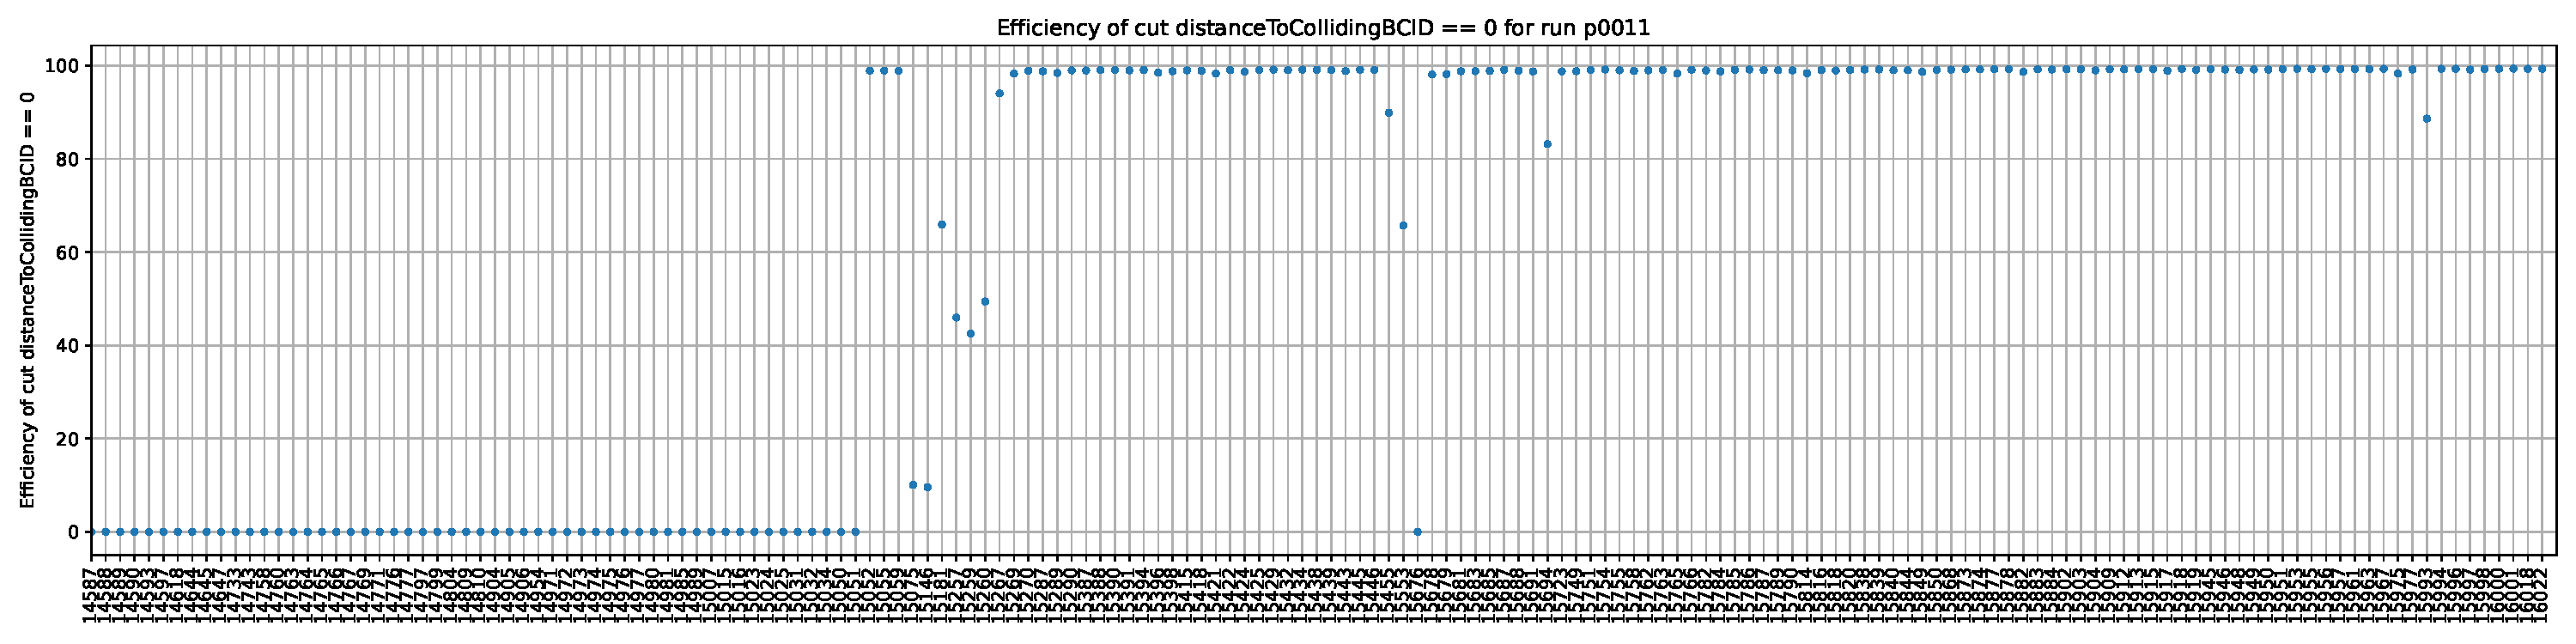
\includegraphics[width=\linewidth]{./assets/BCIDEfficiency_p0011.pdf}
		\caption{Efficiency of the BCID cut on the p0011 data}
	\end{figure}

\end{frame}

\begin{frame}{Yield Plots for F241-2024}
	\begin{figure}
		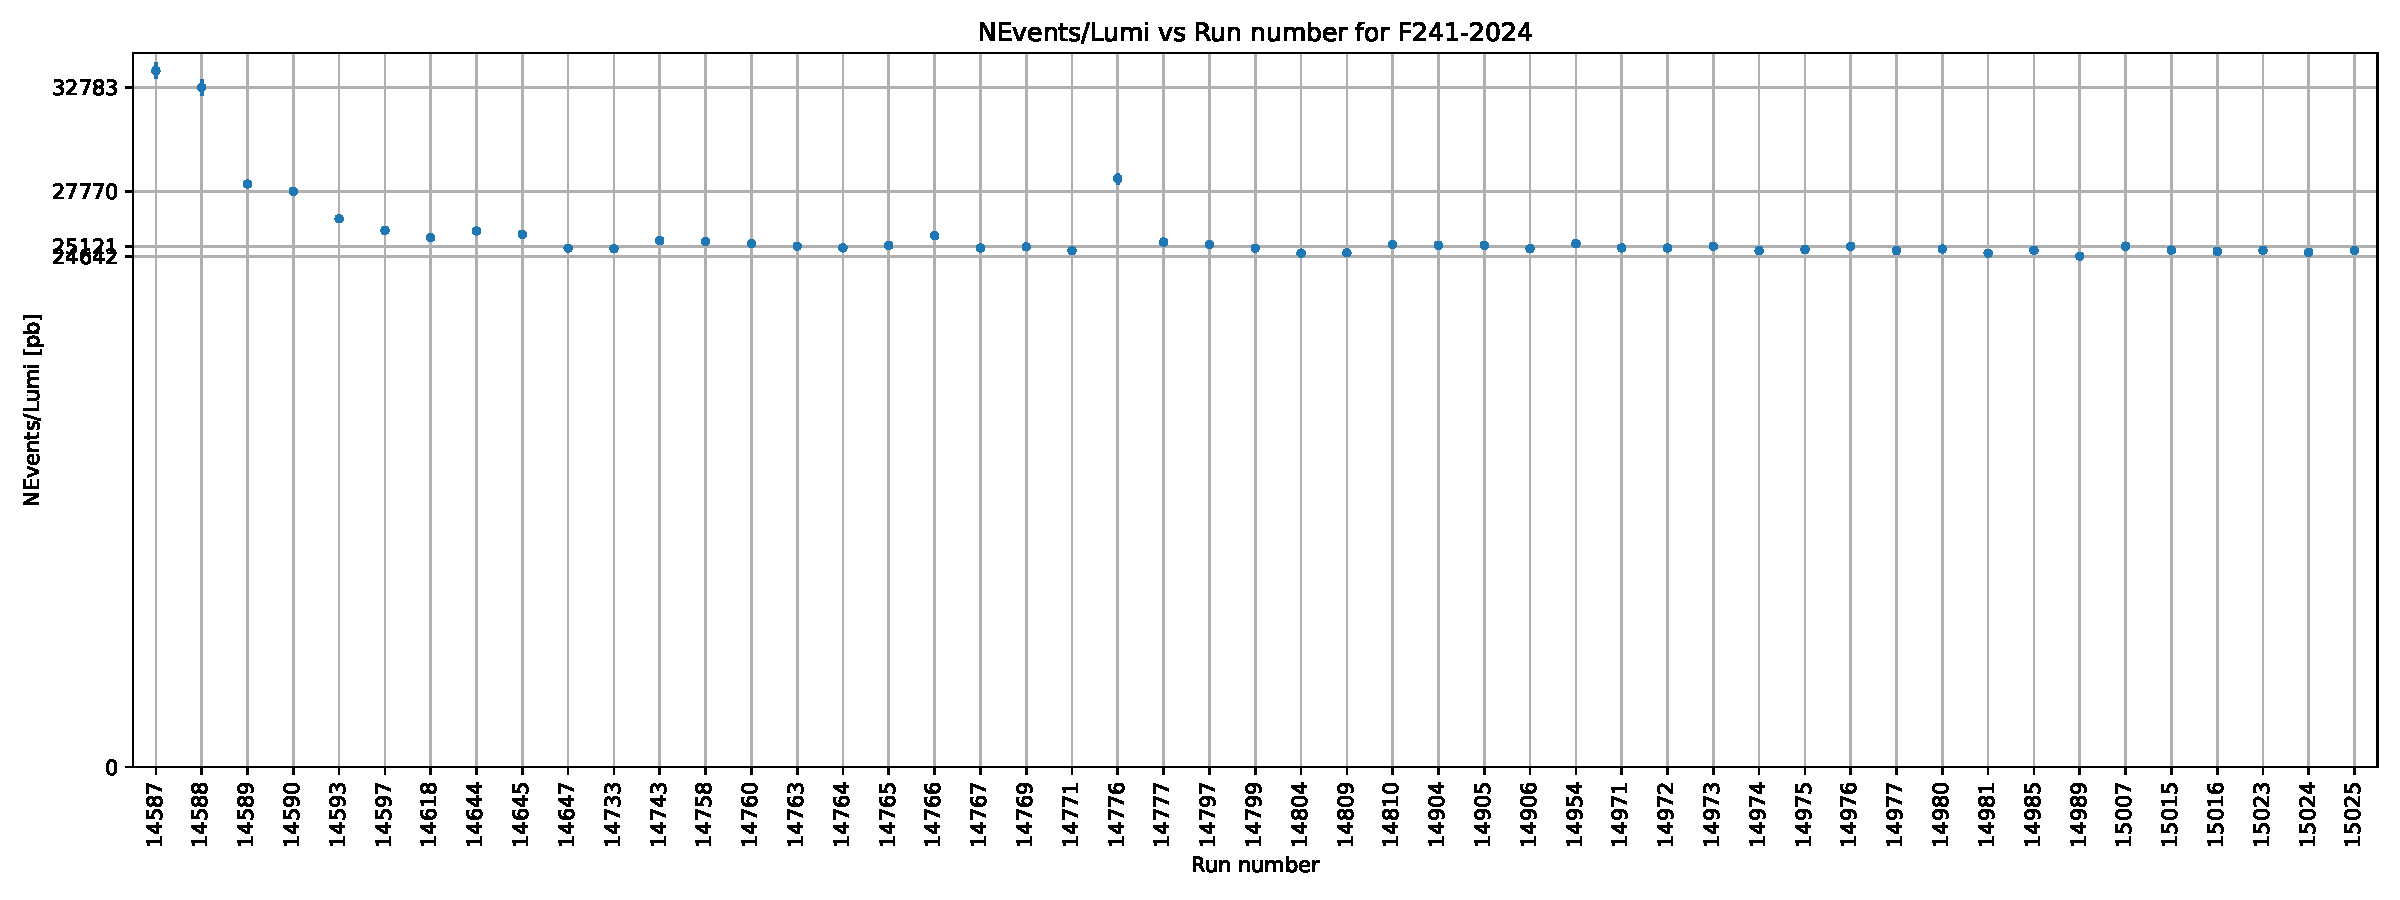
\includegraphics[height=0.4\textheight]{RunwisePlots/F241-2024_NEventsbyLumi.pdf}
	\end{figure}
	\begin{figure}
		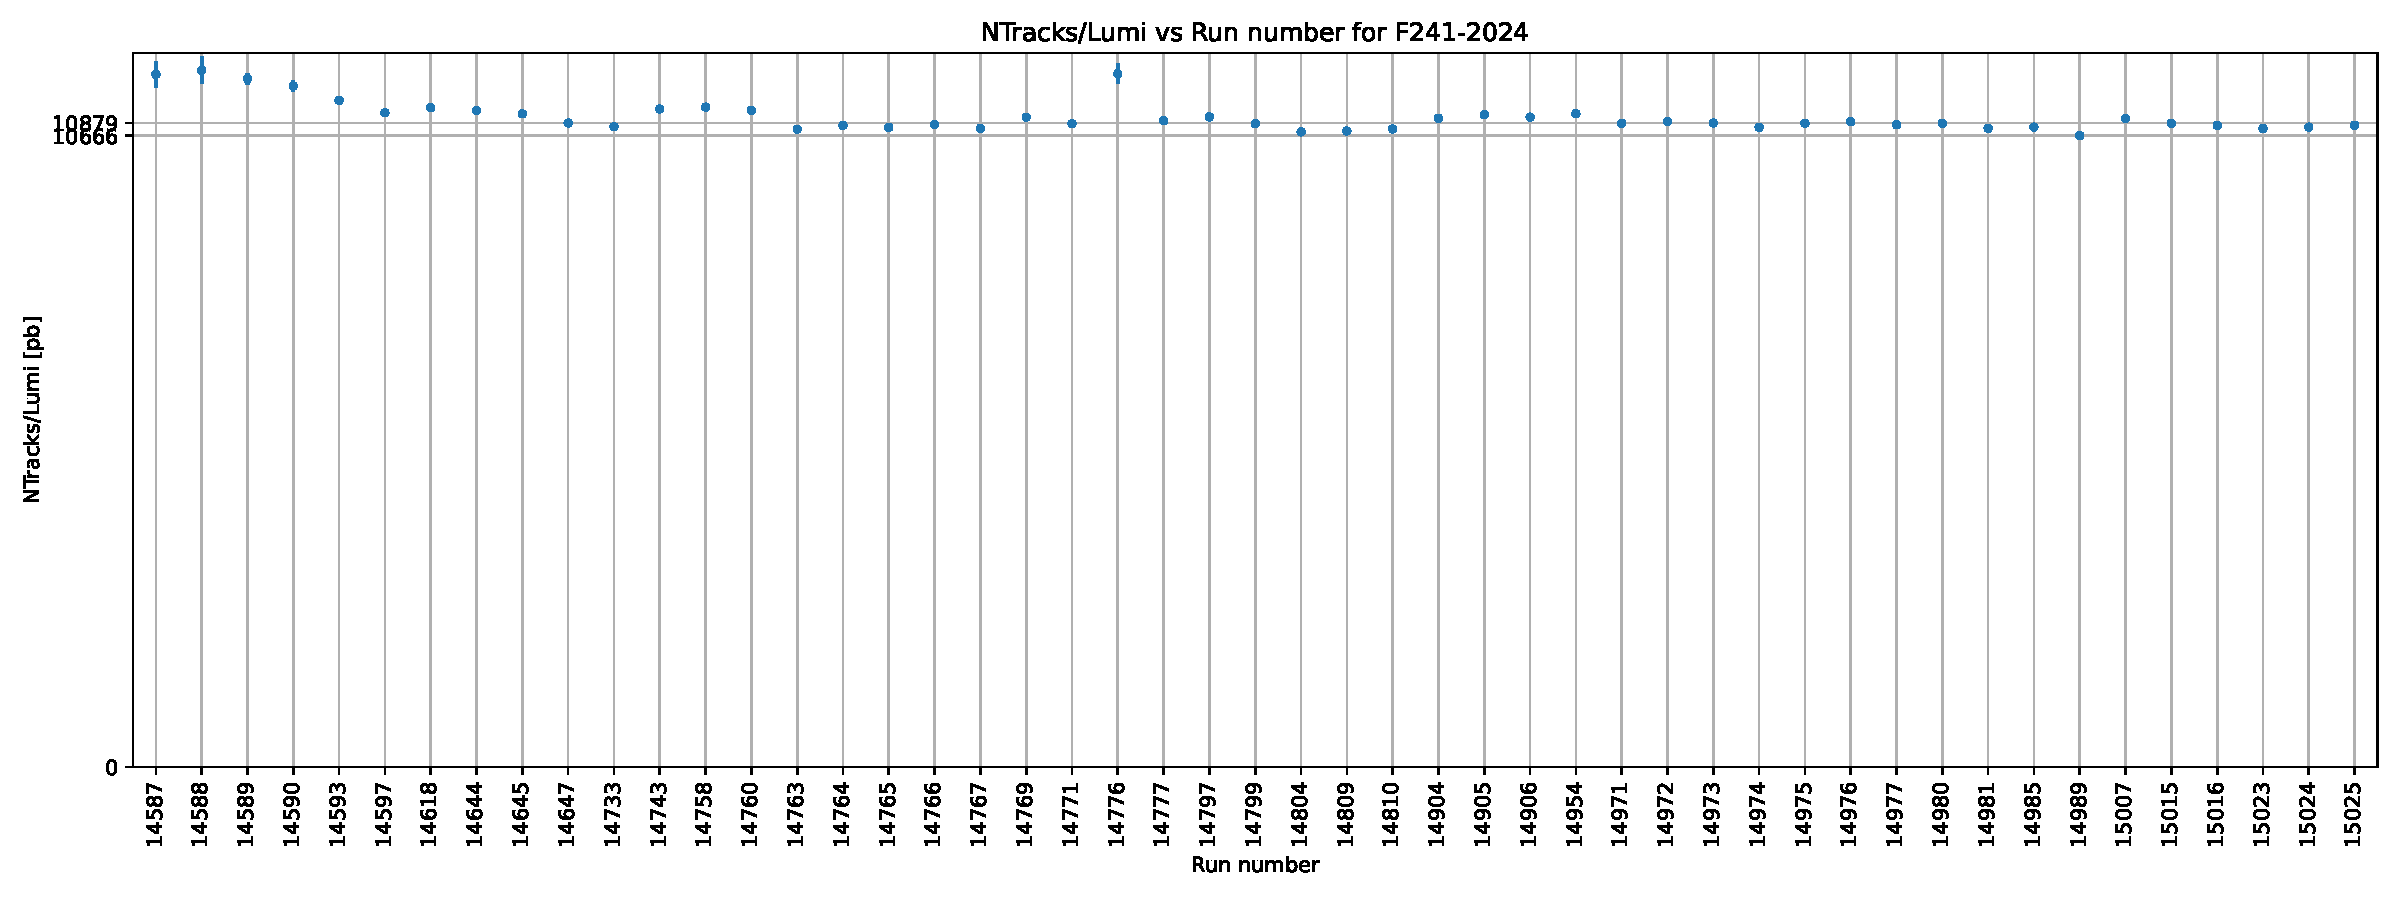
\includegraphics[height=0.4\textheight]{RunwisePlots/F241-2024_NTracksbyLumi.pdf}
	\end{figure}
\end{frame}

\begin{frame}{Yield Plots for Tungsten-2024}
	\begin{figure}
		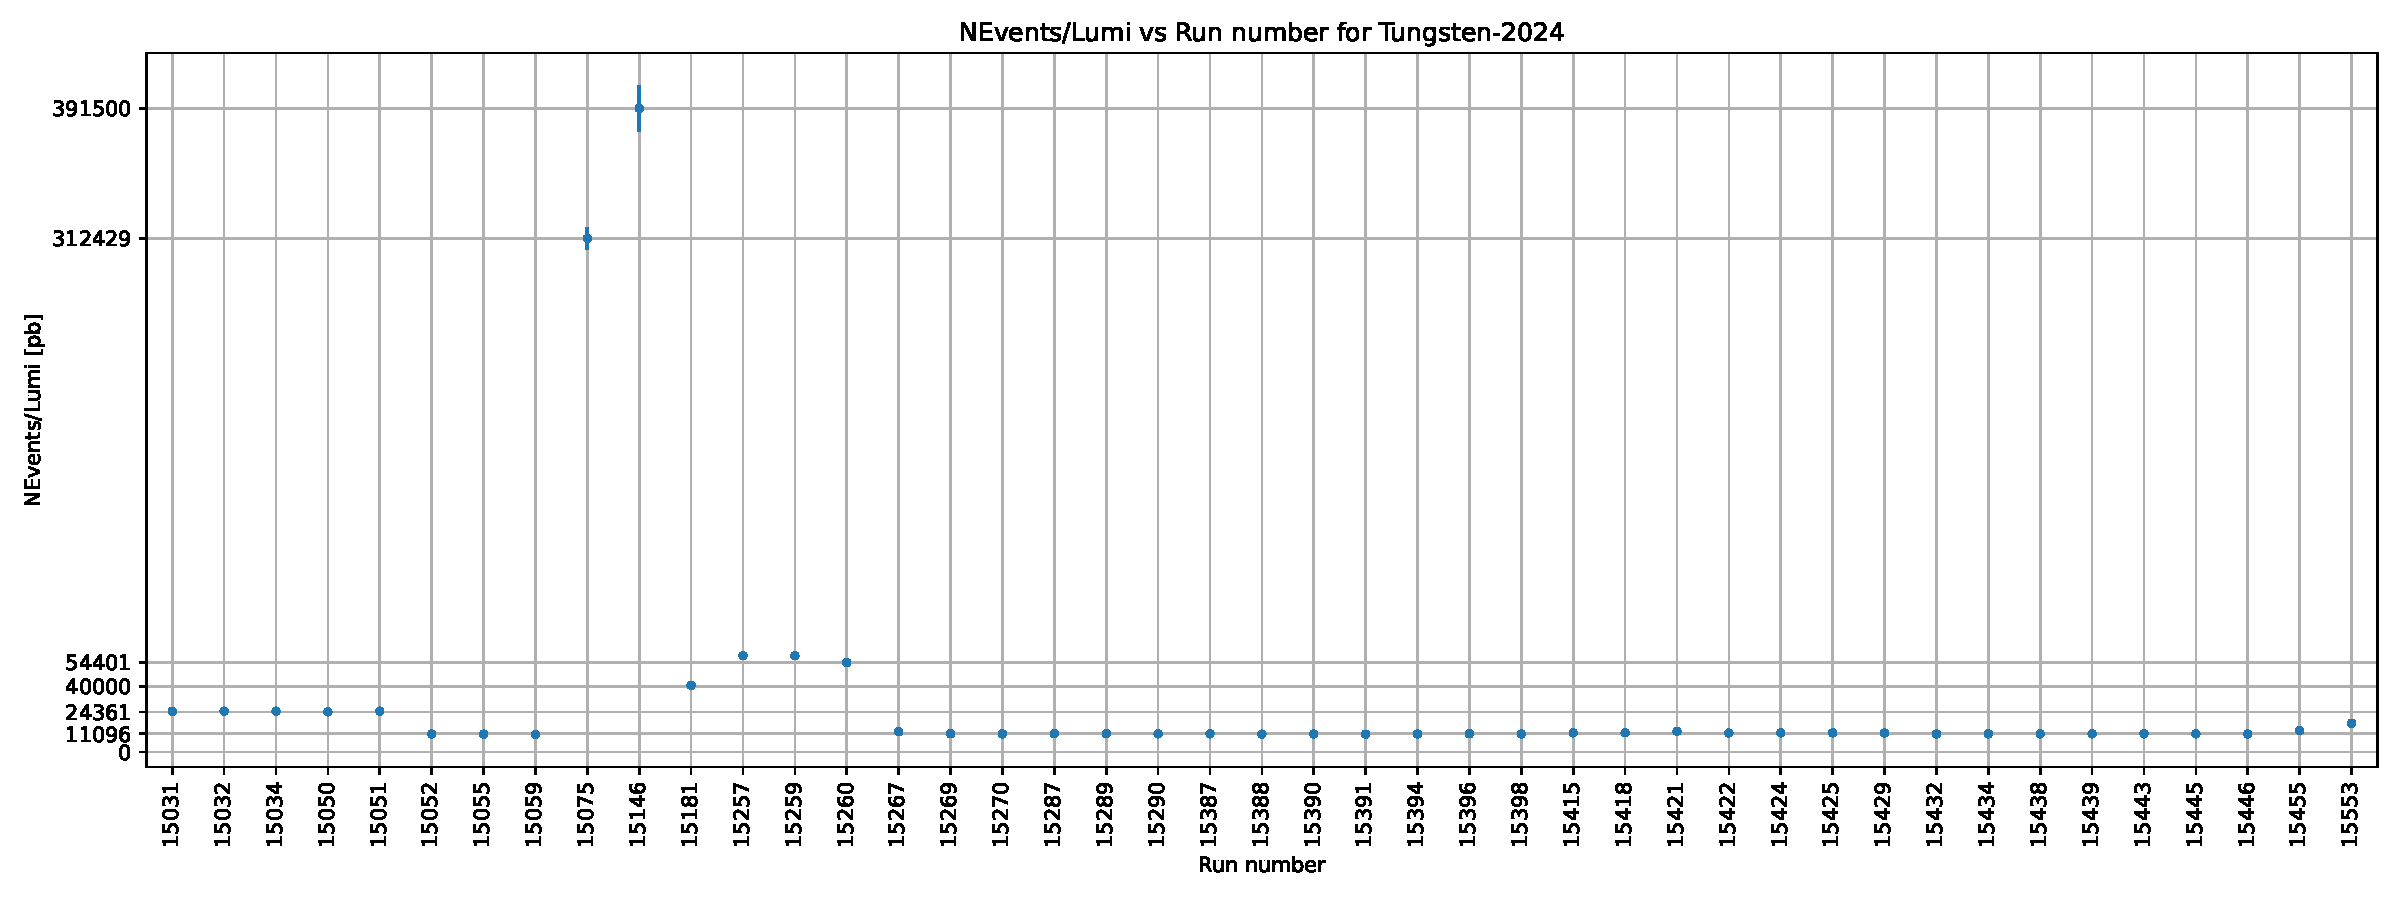
\includegraphics[height=0.4\textheight]{RunwisePlots/Tungsten-2024_NEventsbyLumi.pdf}
	\end{figure}
	\begin{figure}
		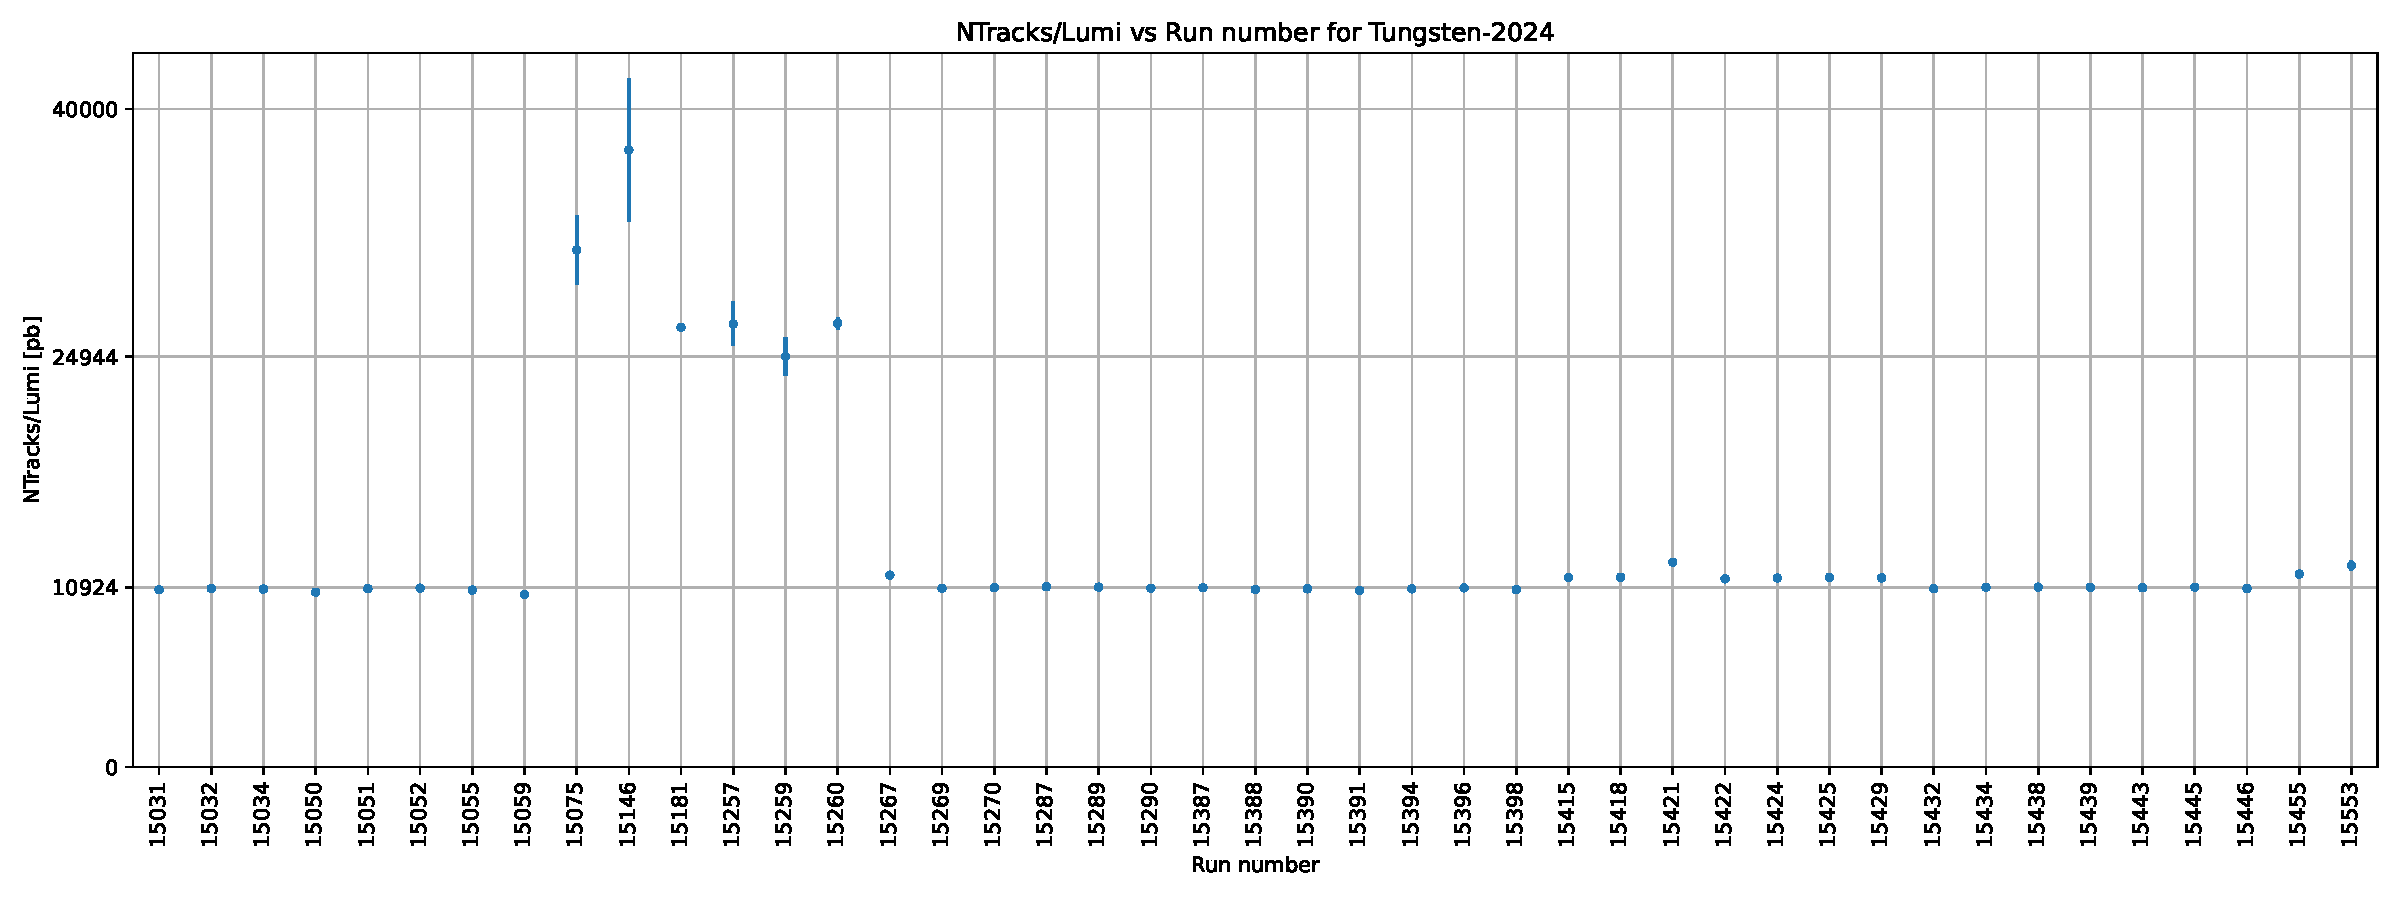
\includegraphics[height=0.4\textheight]{RunwisePlots/Tungsten-2024_NTracksbyLumi.pdf}
	\end{figure}
\end{frame}

\begin{frame}{Yield Plots for F242-2024}
	\begin{figure}
		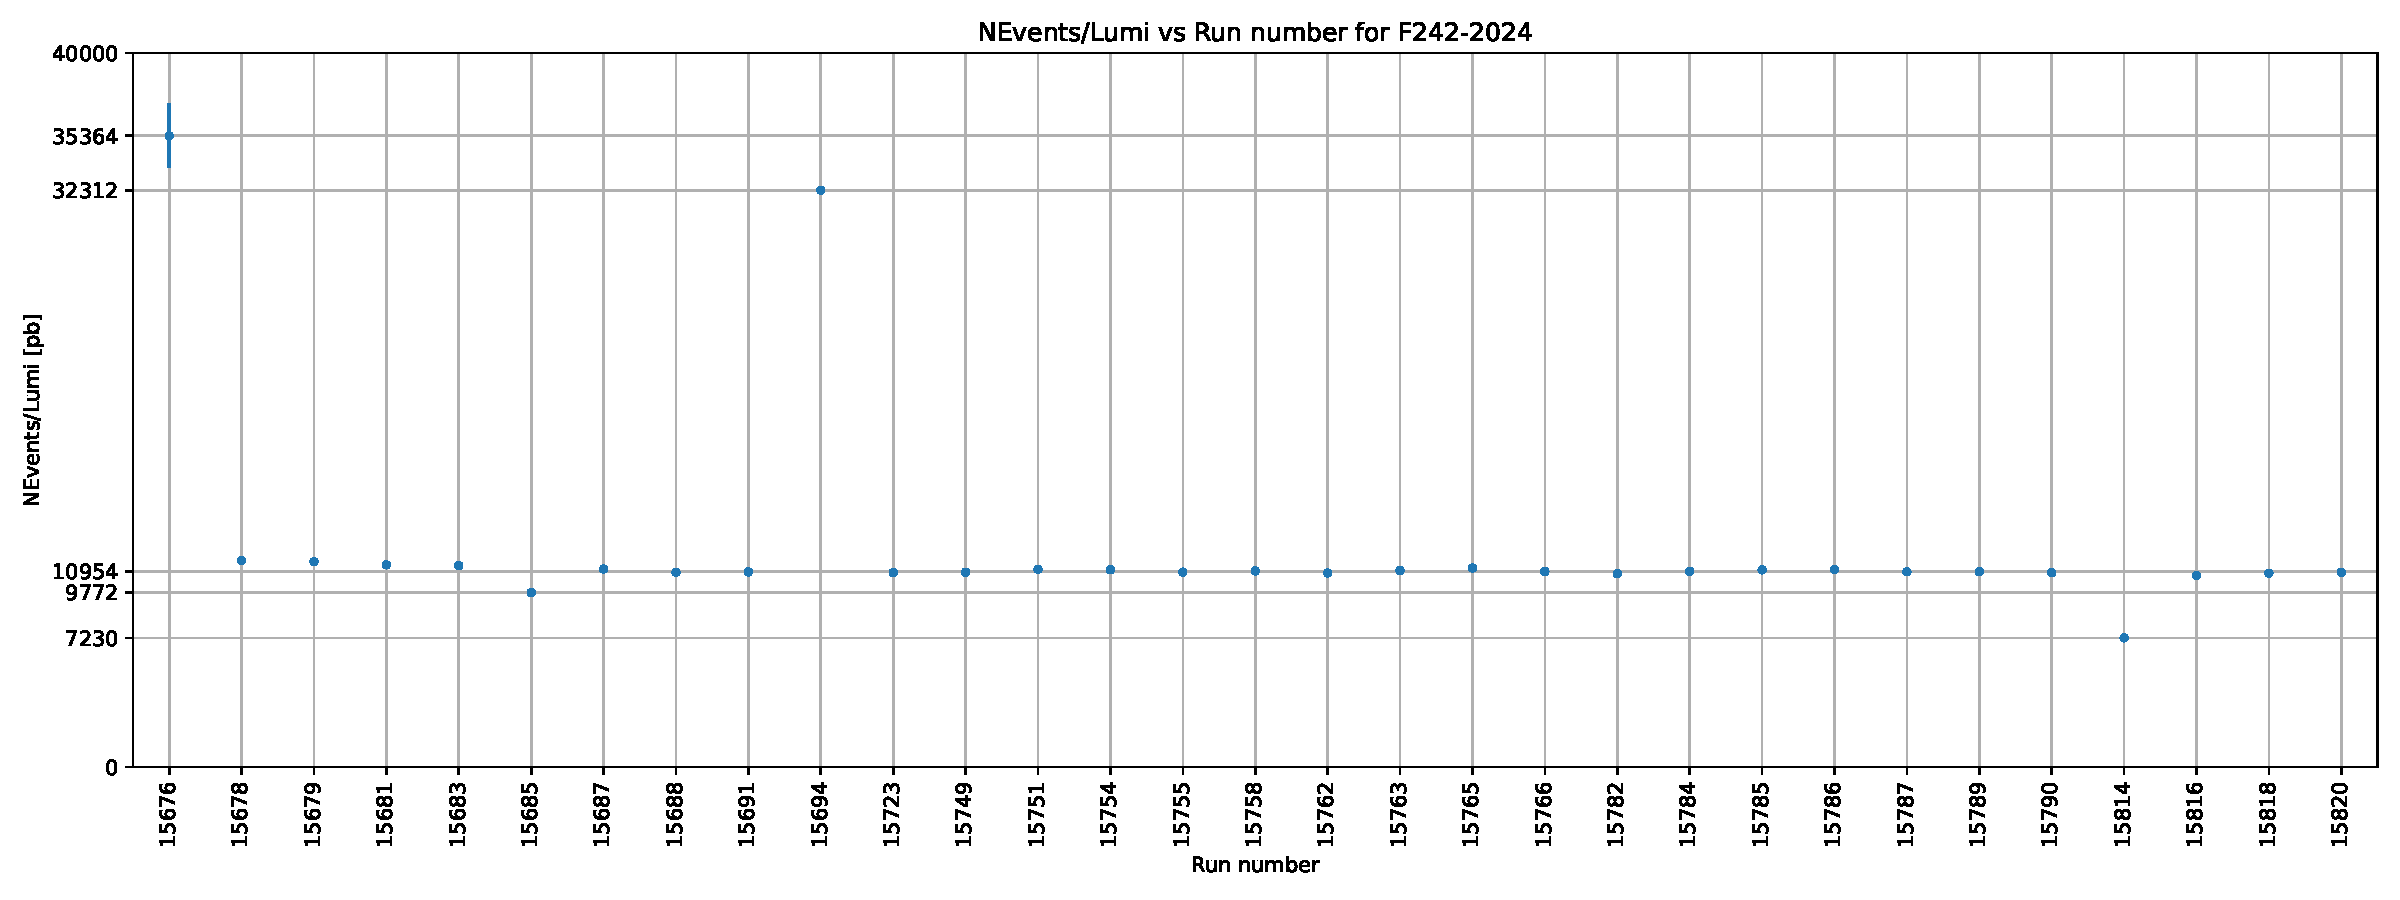
\includegraphics[height=0.4\textheight]{RunwisePlots/F242-2024_NEventsbyLumi.pdf}
	\end{figure}
	\begin{figure}
		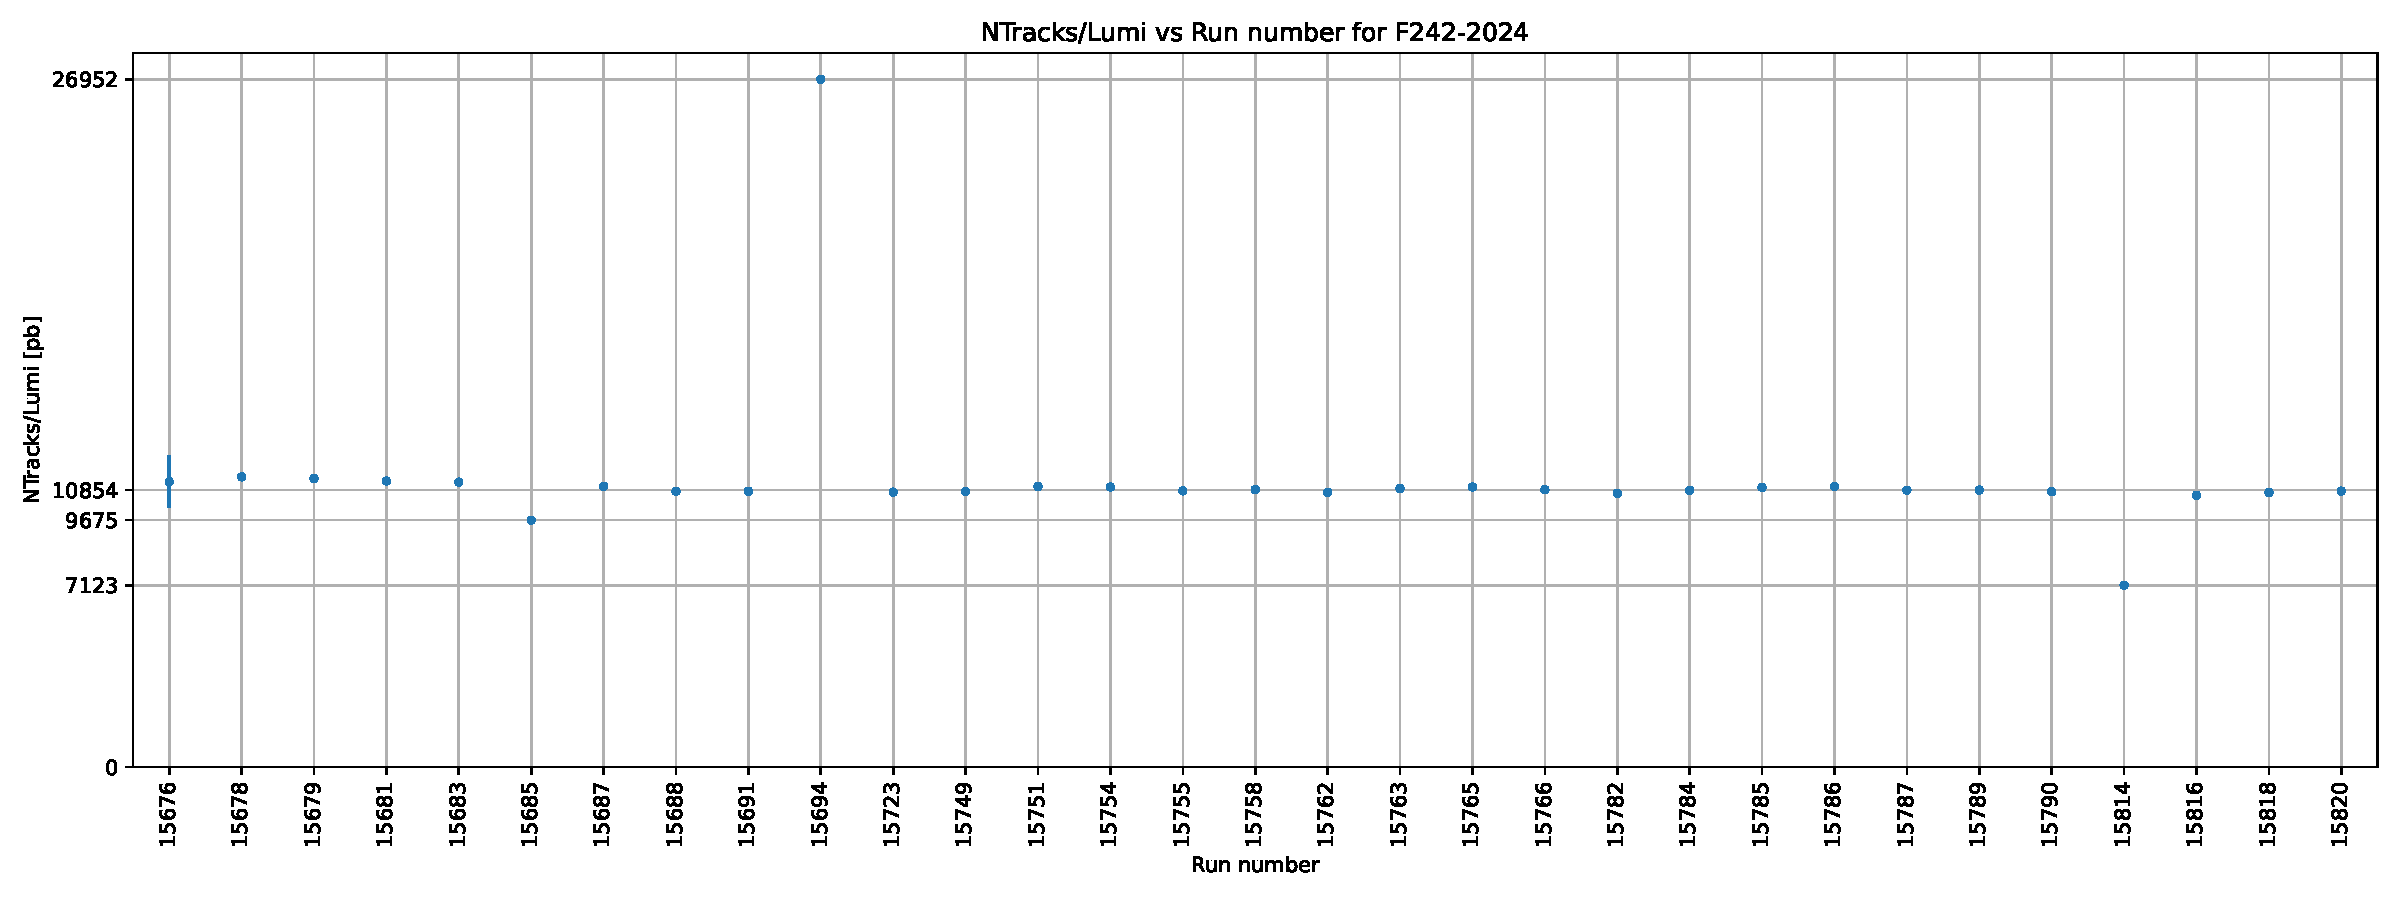
\includegraphics[height=0.4\textheight]{RunwisePlots/F242-2024_NTracksbyLumi.pdf}
	\end{figure}
\end{frame}

\begin{frame}{Yield Plots for CaloNu-2024}
	\begin{figure}
		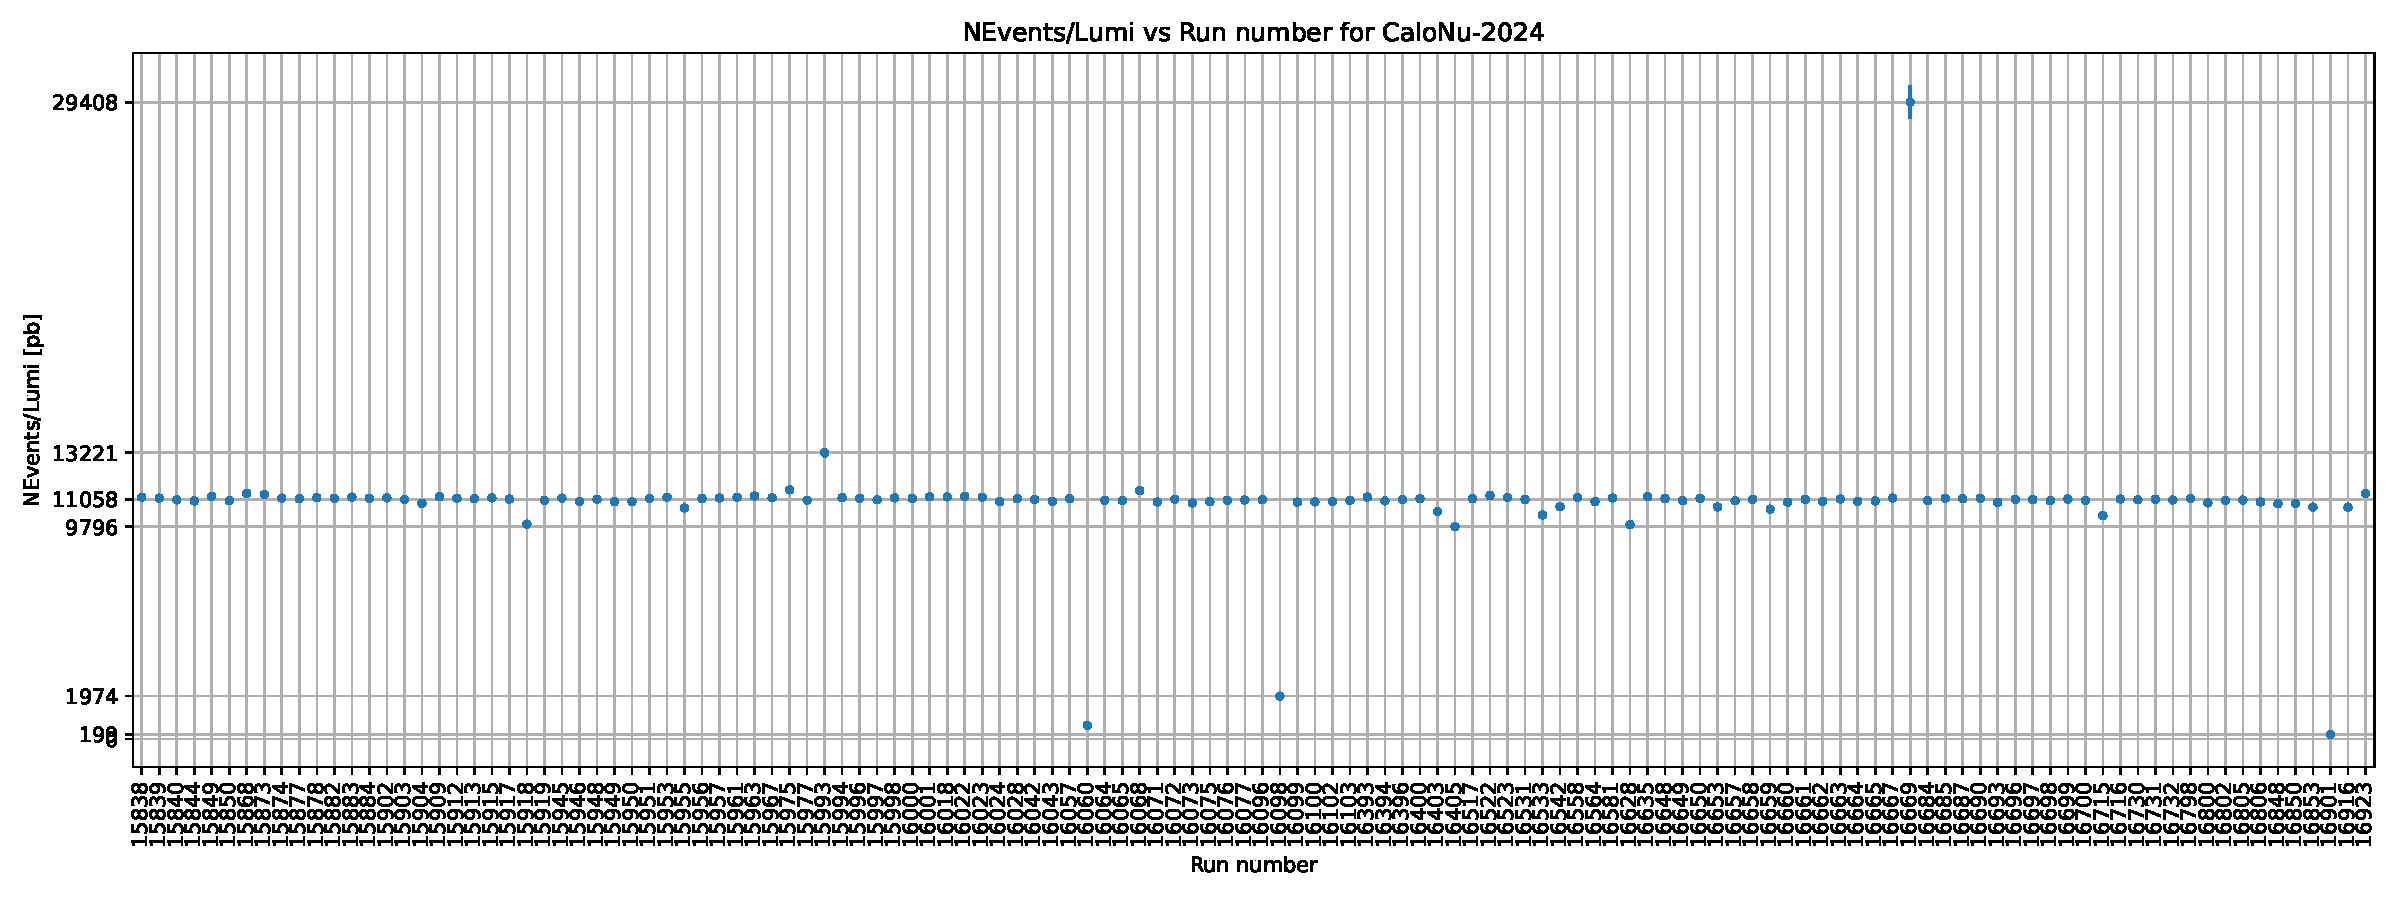
\includegraphics[height=0.4\textheight]{RunwisePlots/CaloNu-2024_NEventsbyLumi.pdf}
	\end{figure}
	\begin{figure}
		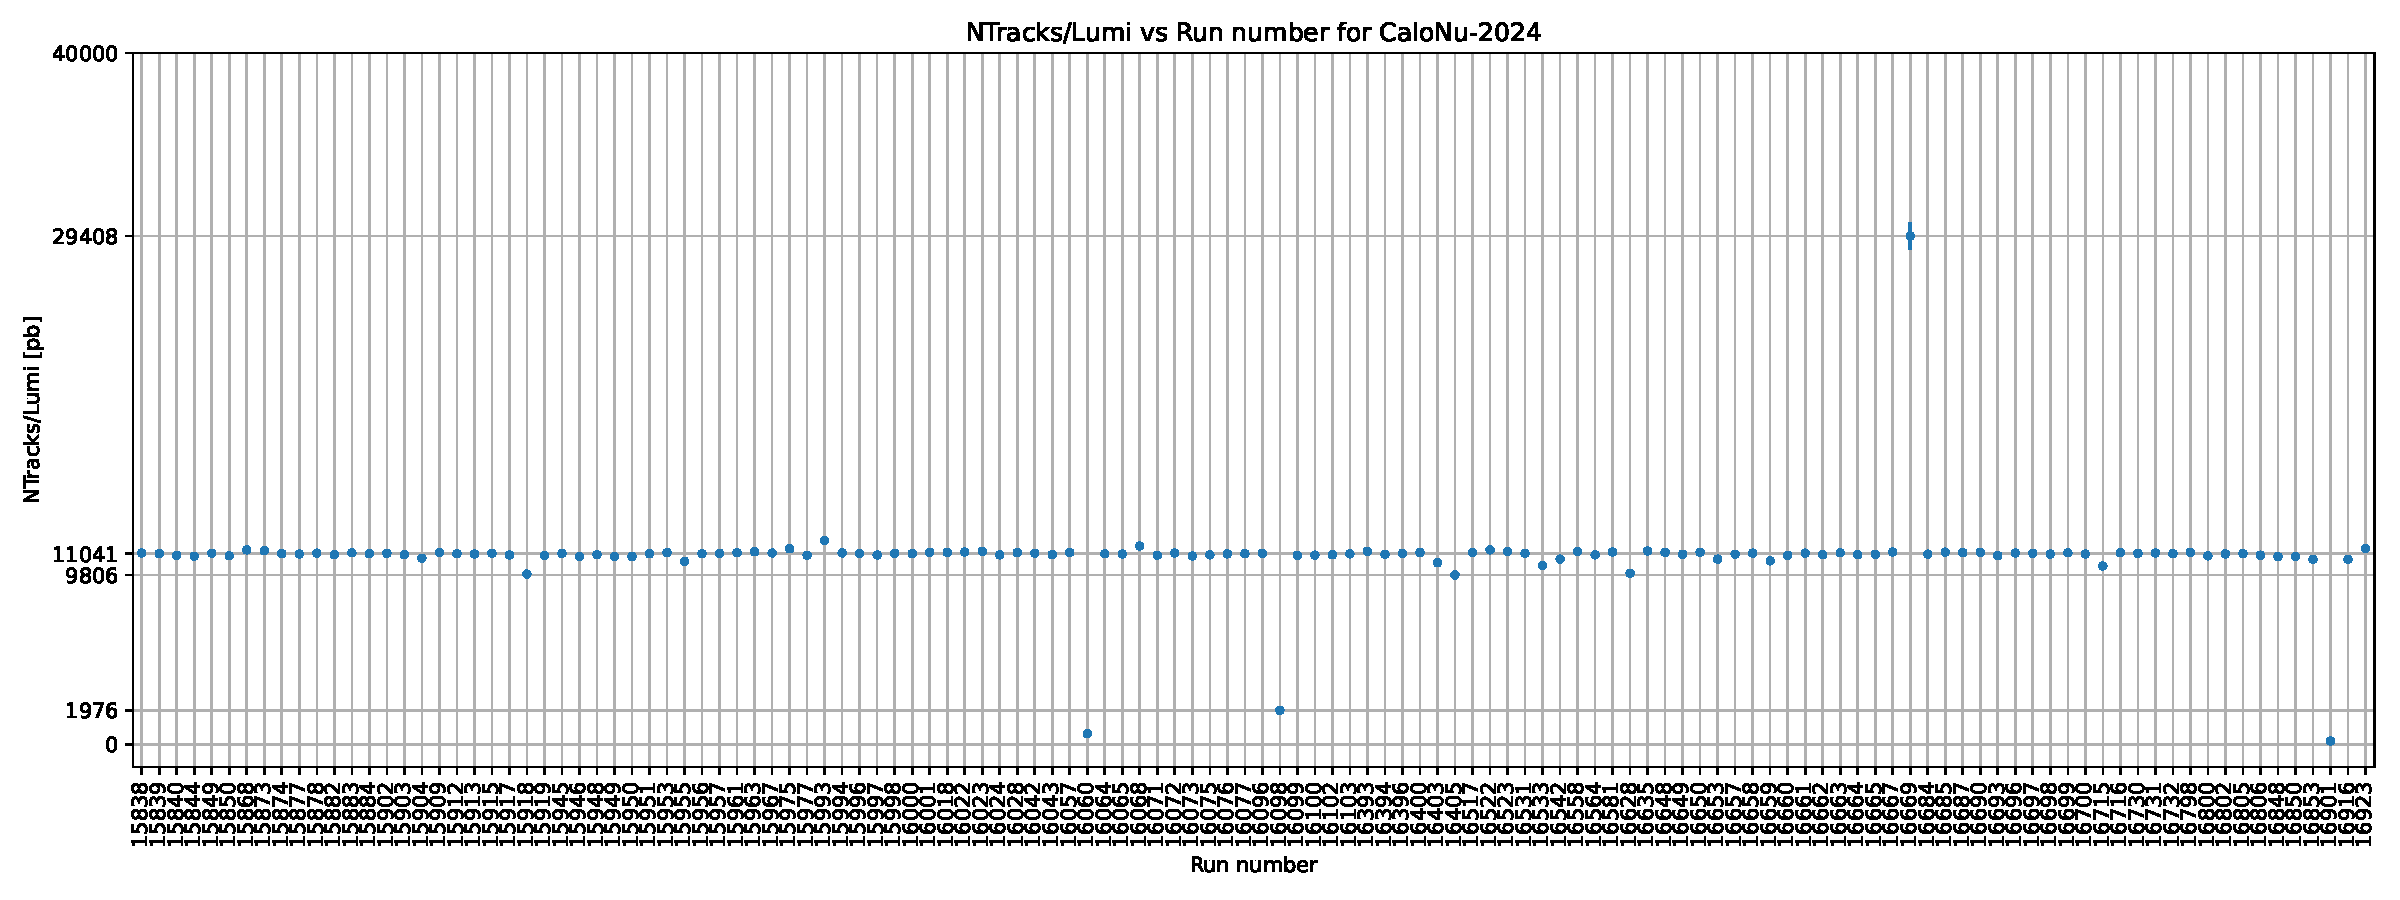
\includegraphics[height=0.4\textheight]{RunwisePlots/CaloNu-2024_NTracksbyLumi.pdf}
	\end{figure}
\end{frame}

\begin{frame}{Yield Plots for F243-2024}
	\begin{figure}
		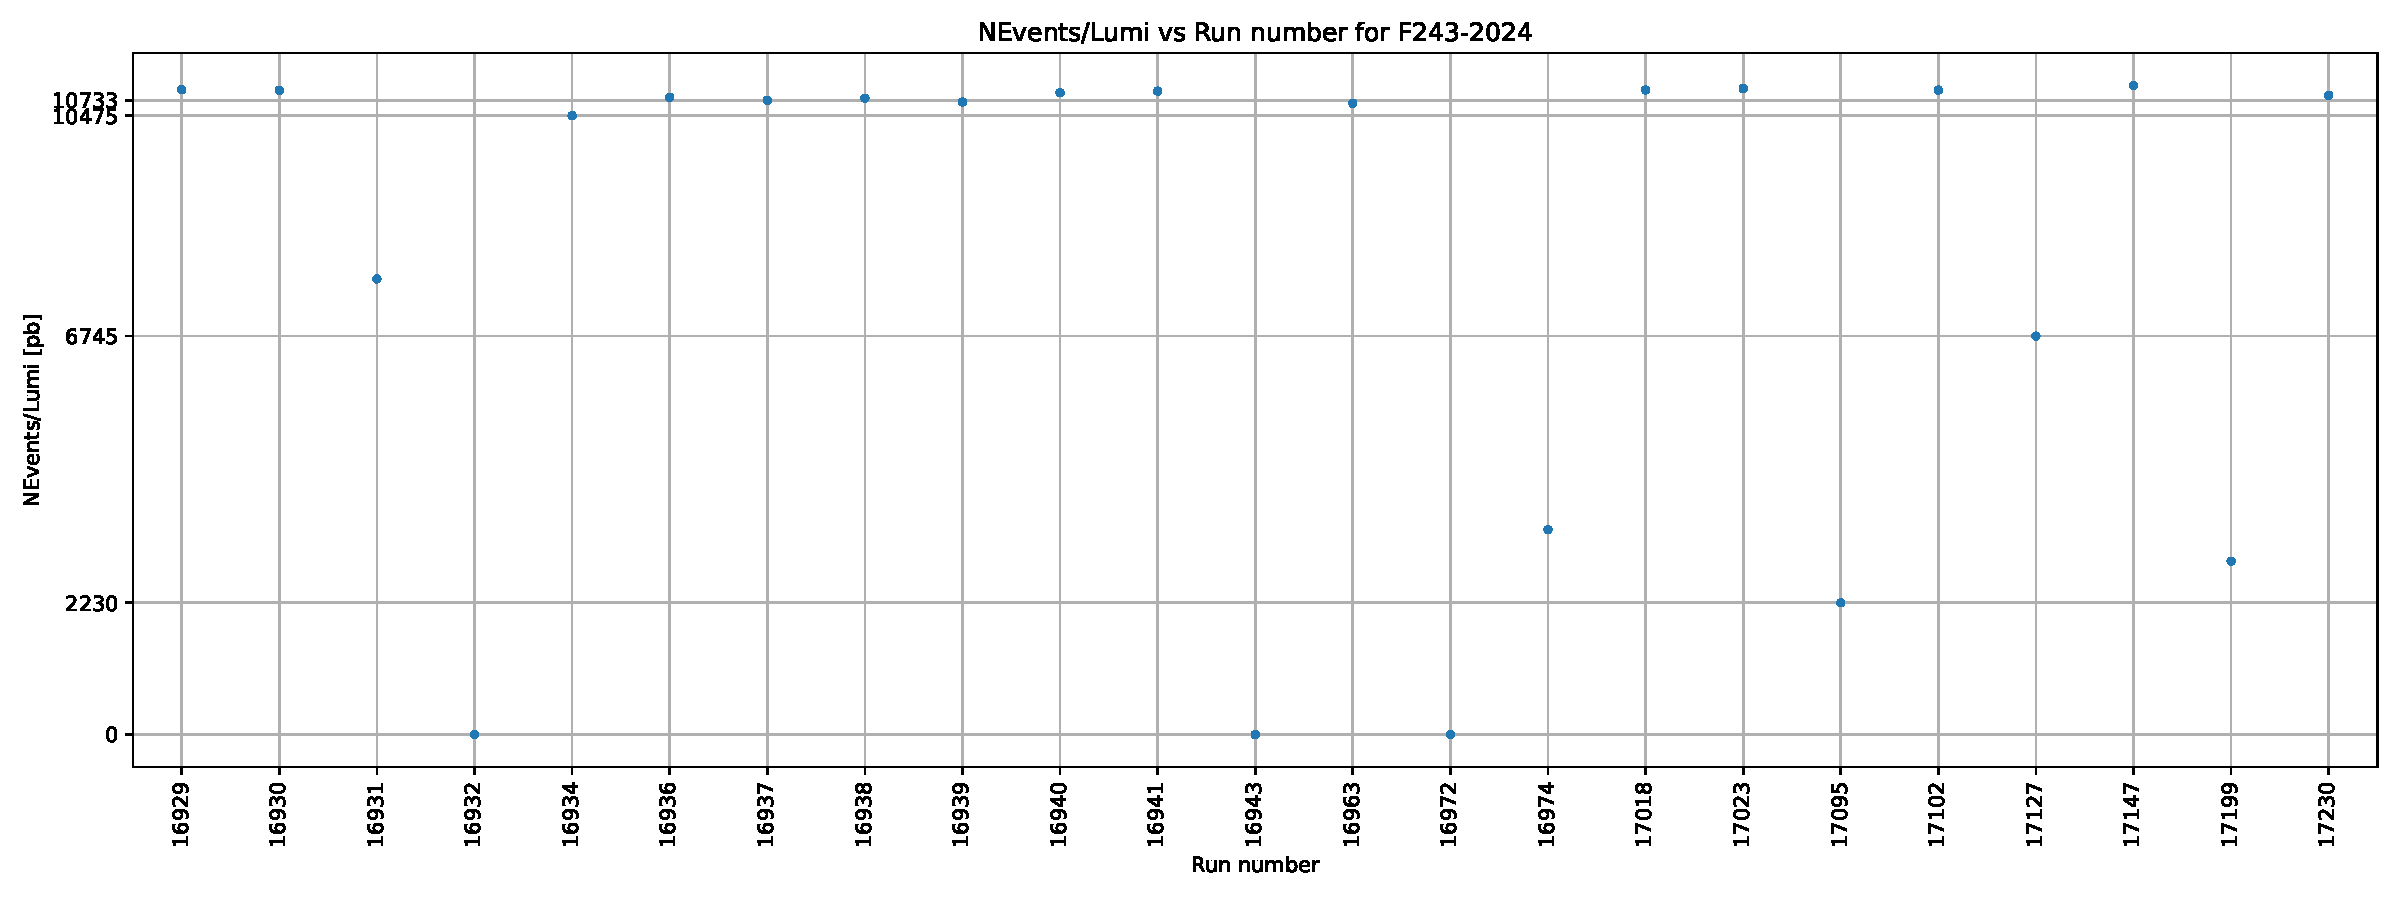
\includegraphics[height=0.4\textheight]{RunwisePlots/F243-2024_NEventsbyLumi.pdf}
	\end{figure}
	\begin{figure}
		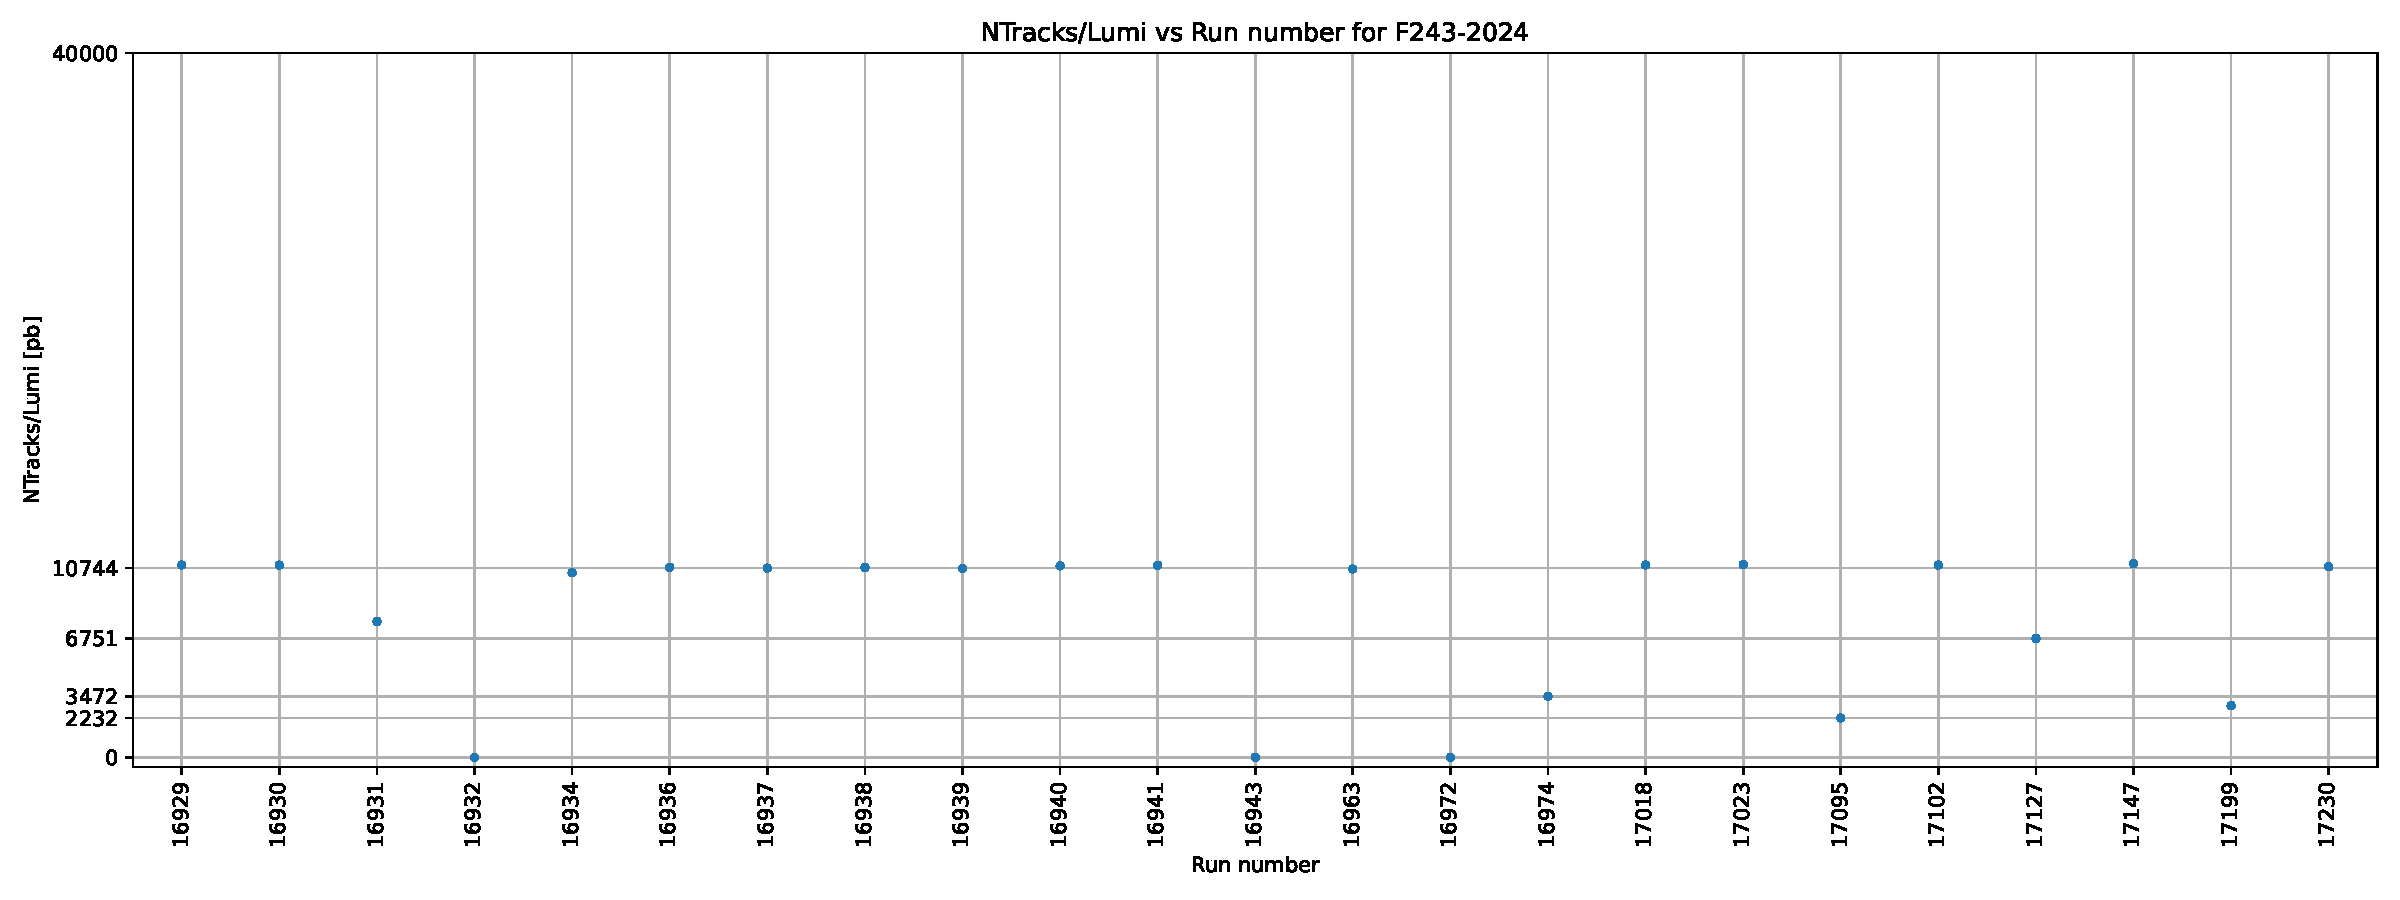
\includegraphics[height=0.4\textheight]{RunwisePlots/F243-2024_NTracksbyLumi.pdf}
	\end{figure}
\end{frame}

\begin{frame}{Median Yeilds across Runs}
	\begin{figure}
		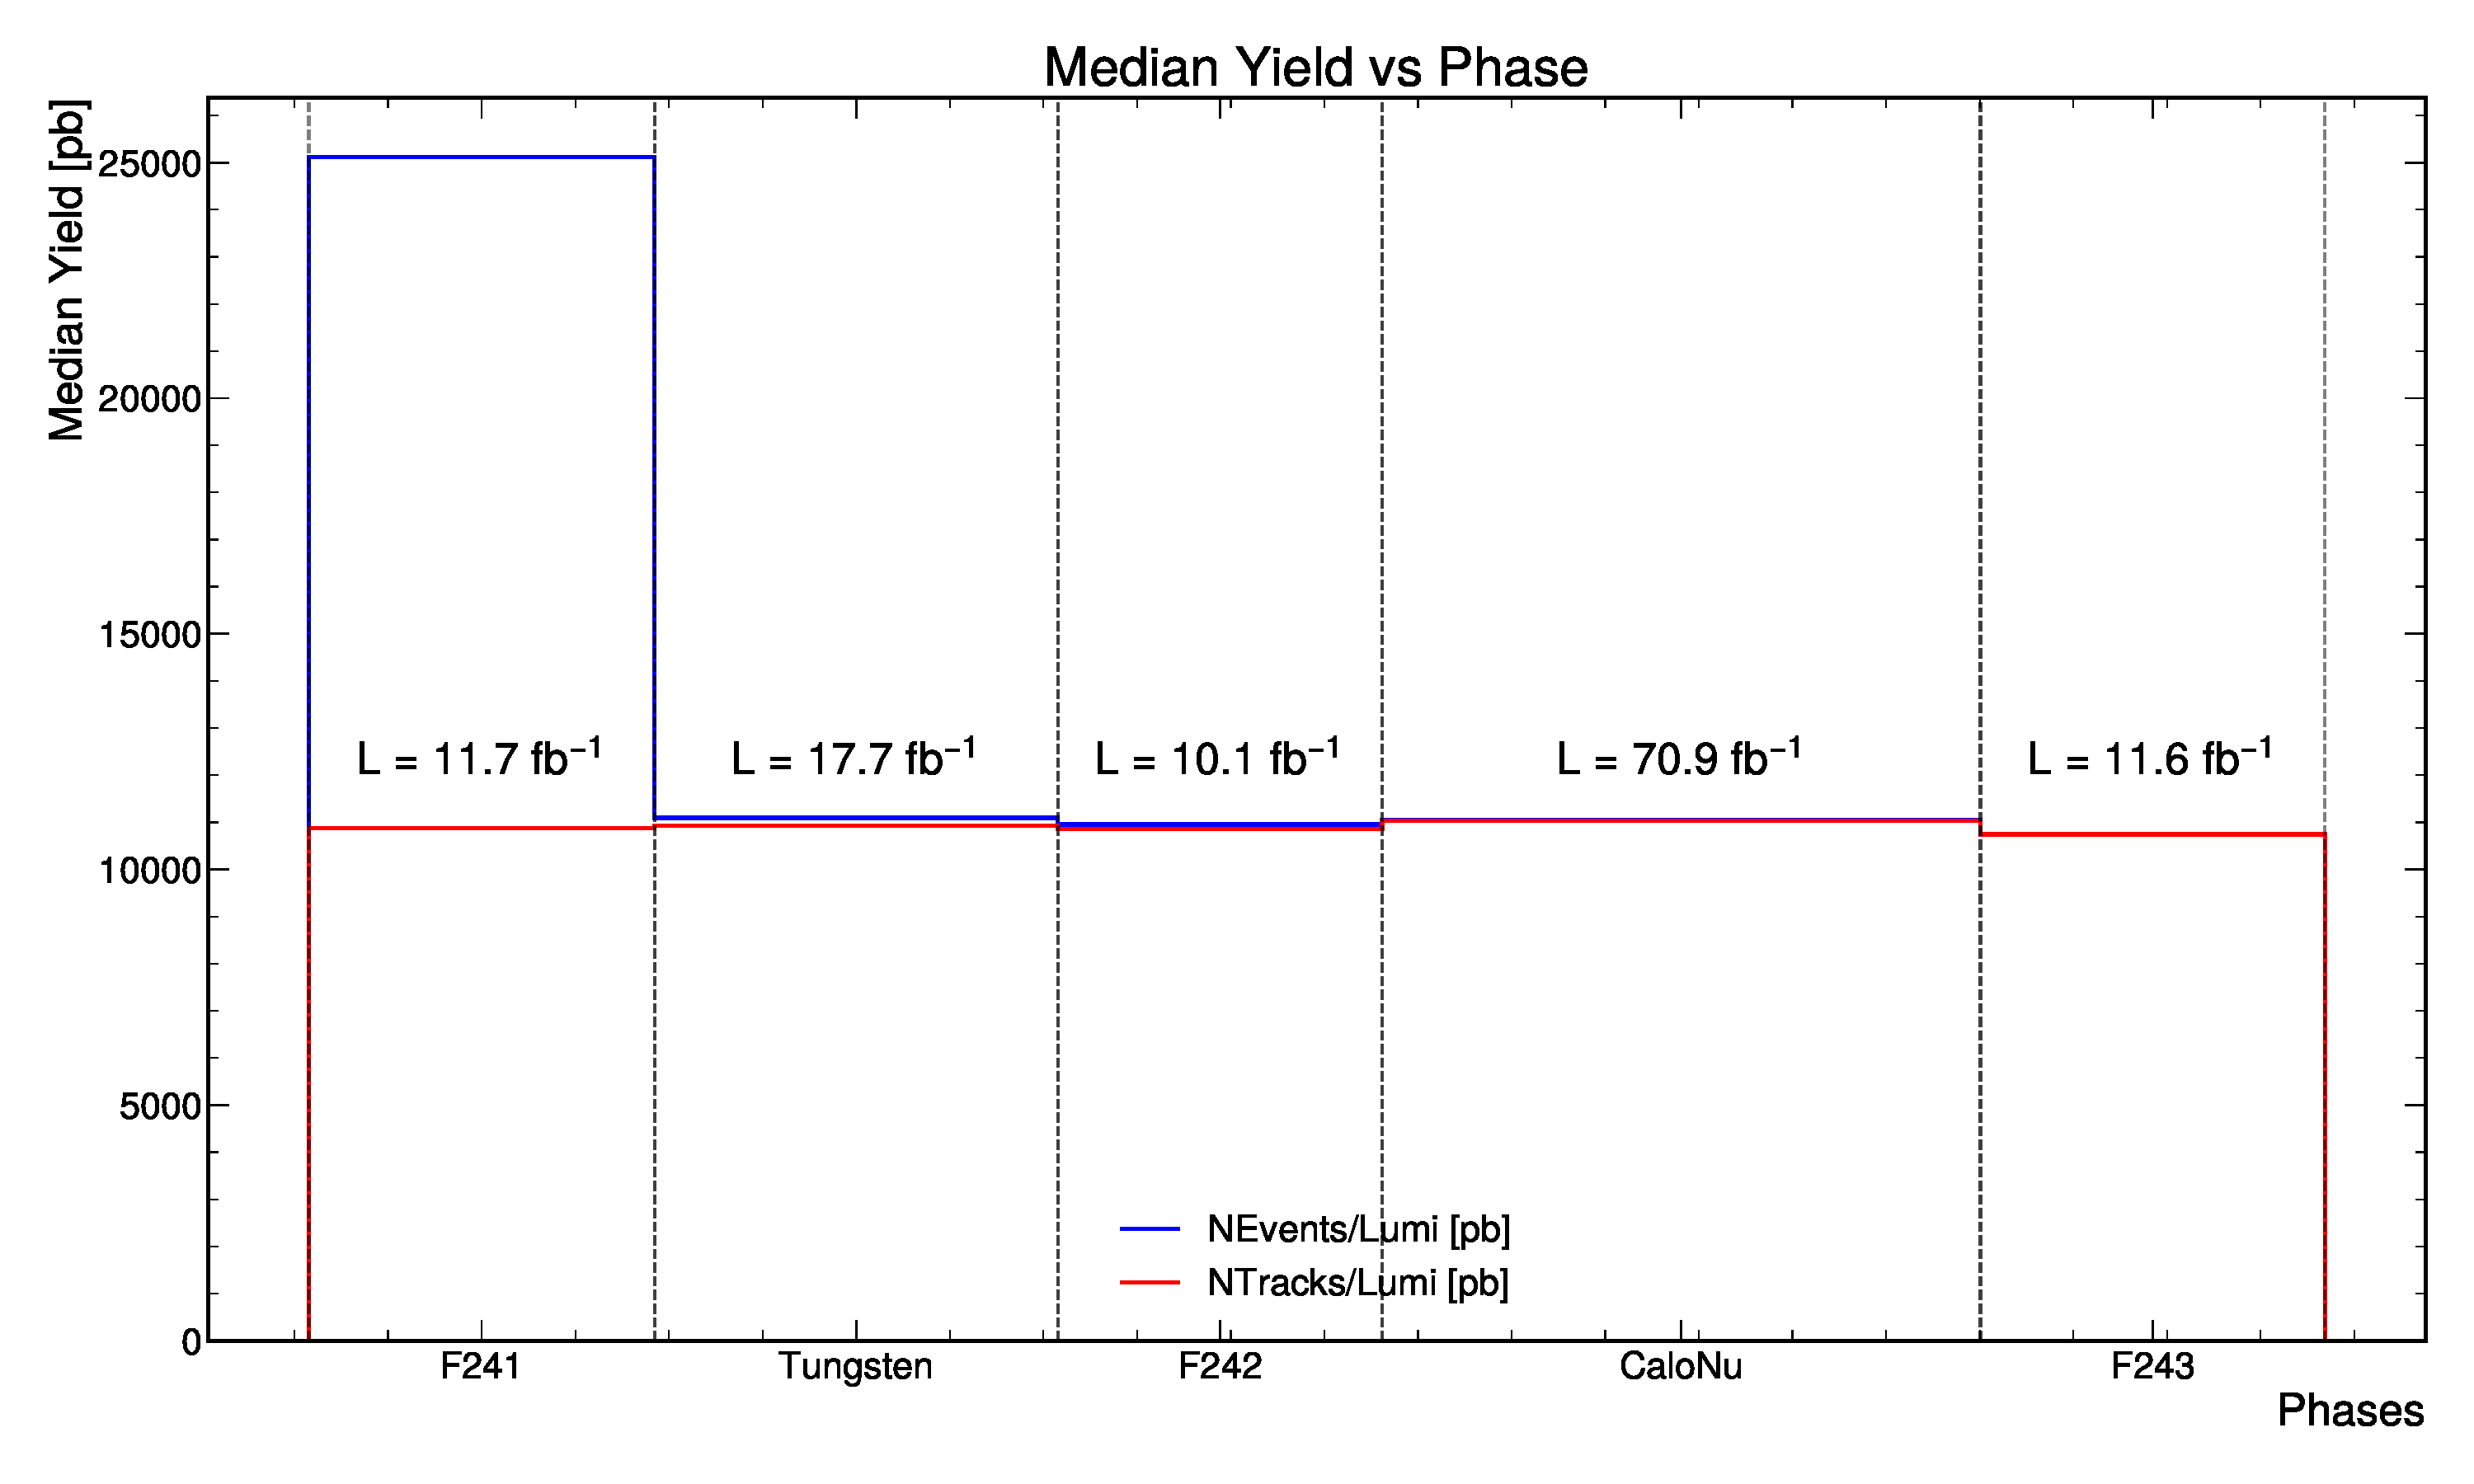
\includegraphics[width=\linewidth]{./RunwisePlots/MedianYieldsPhase.pdf}
	\end{figure}
	\vspace{-0.5cm}
	\begin{itemize}
		\item Possible anomaly in the F241 data?
	\end{itemize}
\end{frame}

\begin{frame}{Distribution of Track Parameters across Runs}
	\begin{center}
		Excellent agreement of variables across runs !
	\end{center}
	
\end{frame}


\begin{frame}{Distribution of Track X0 across 2024 runs}
	\begin{figure}
		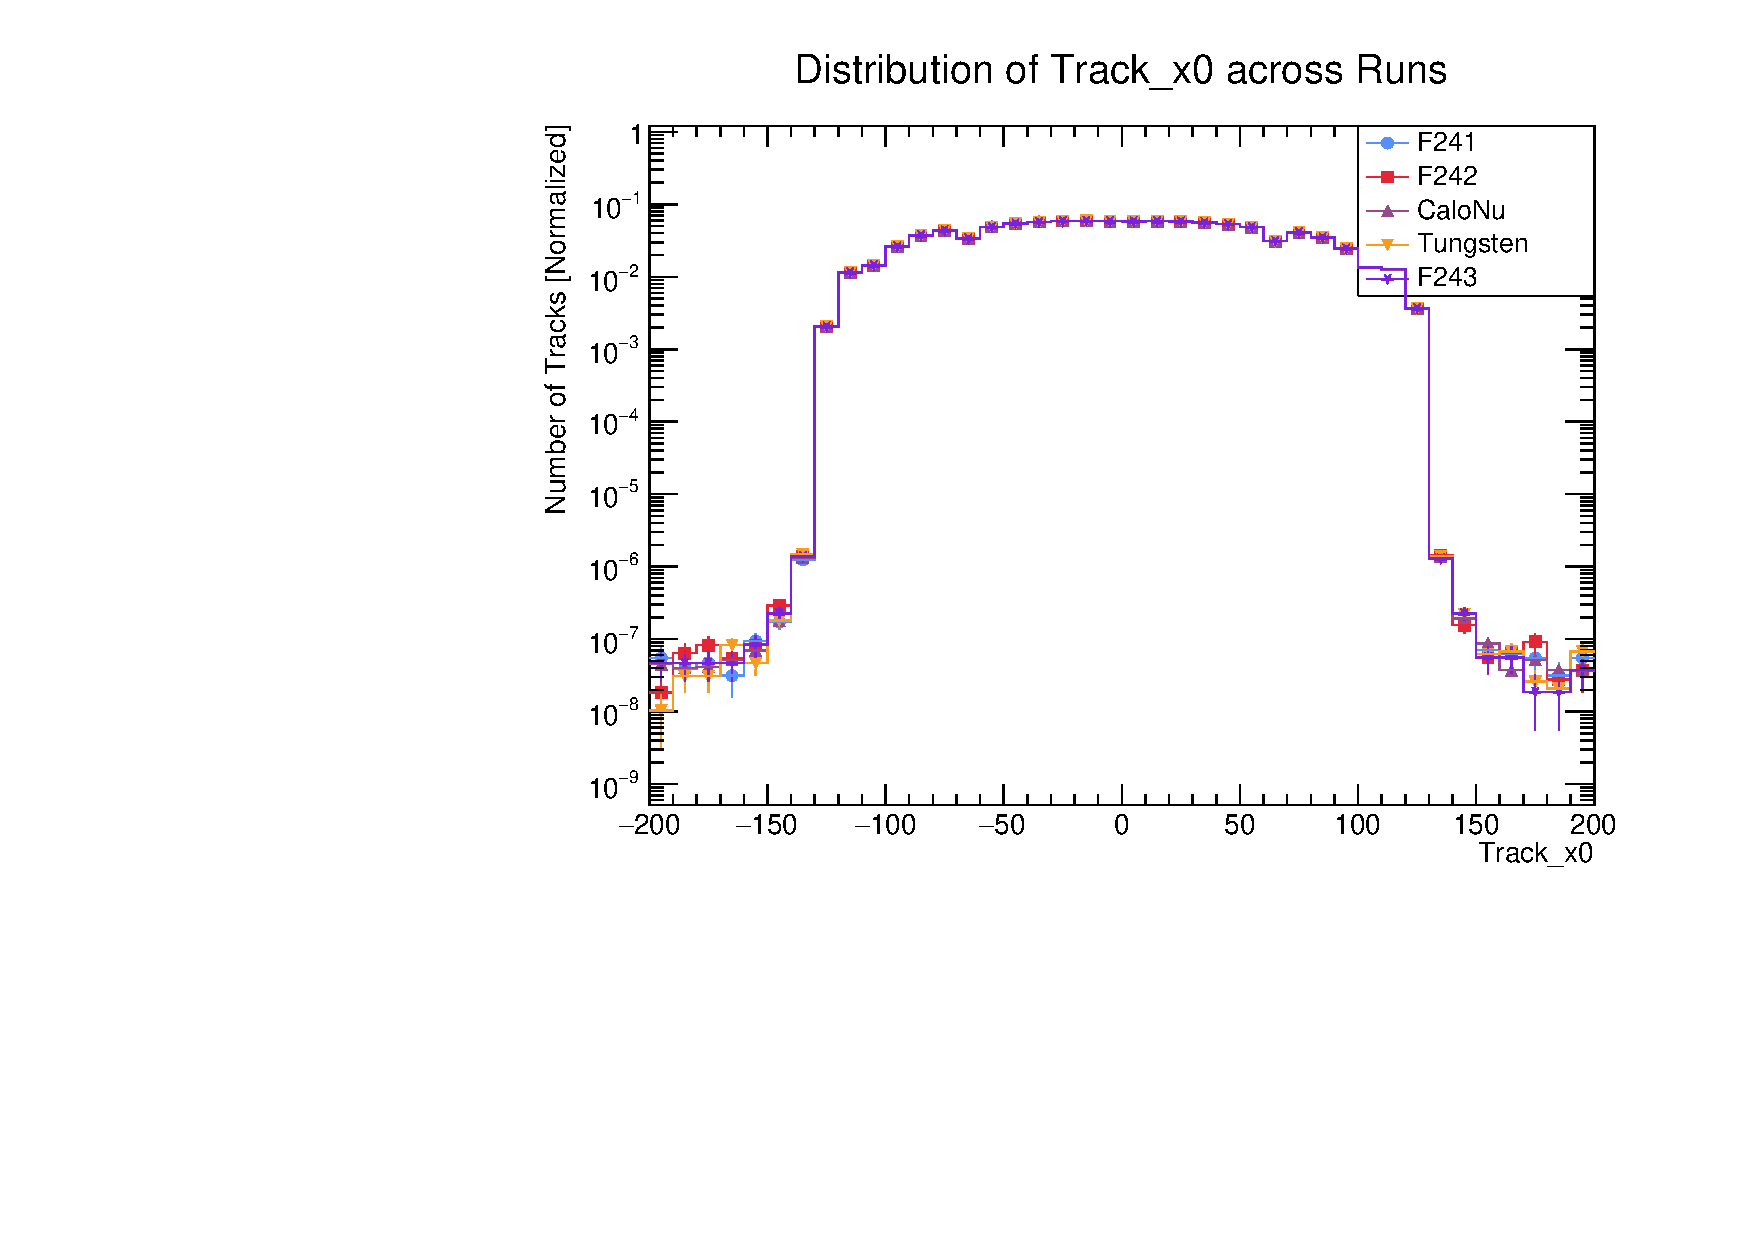
\includegraphics[width=\linewidth]{./RunwisePlots/Track_x0_runwise.pdf}
	\end{figure}
\end{frame}
\begin{frame}{Distribution of Track Y0 across runs}
	\begin{figure}
		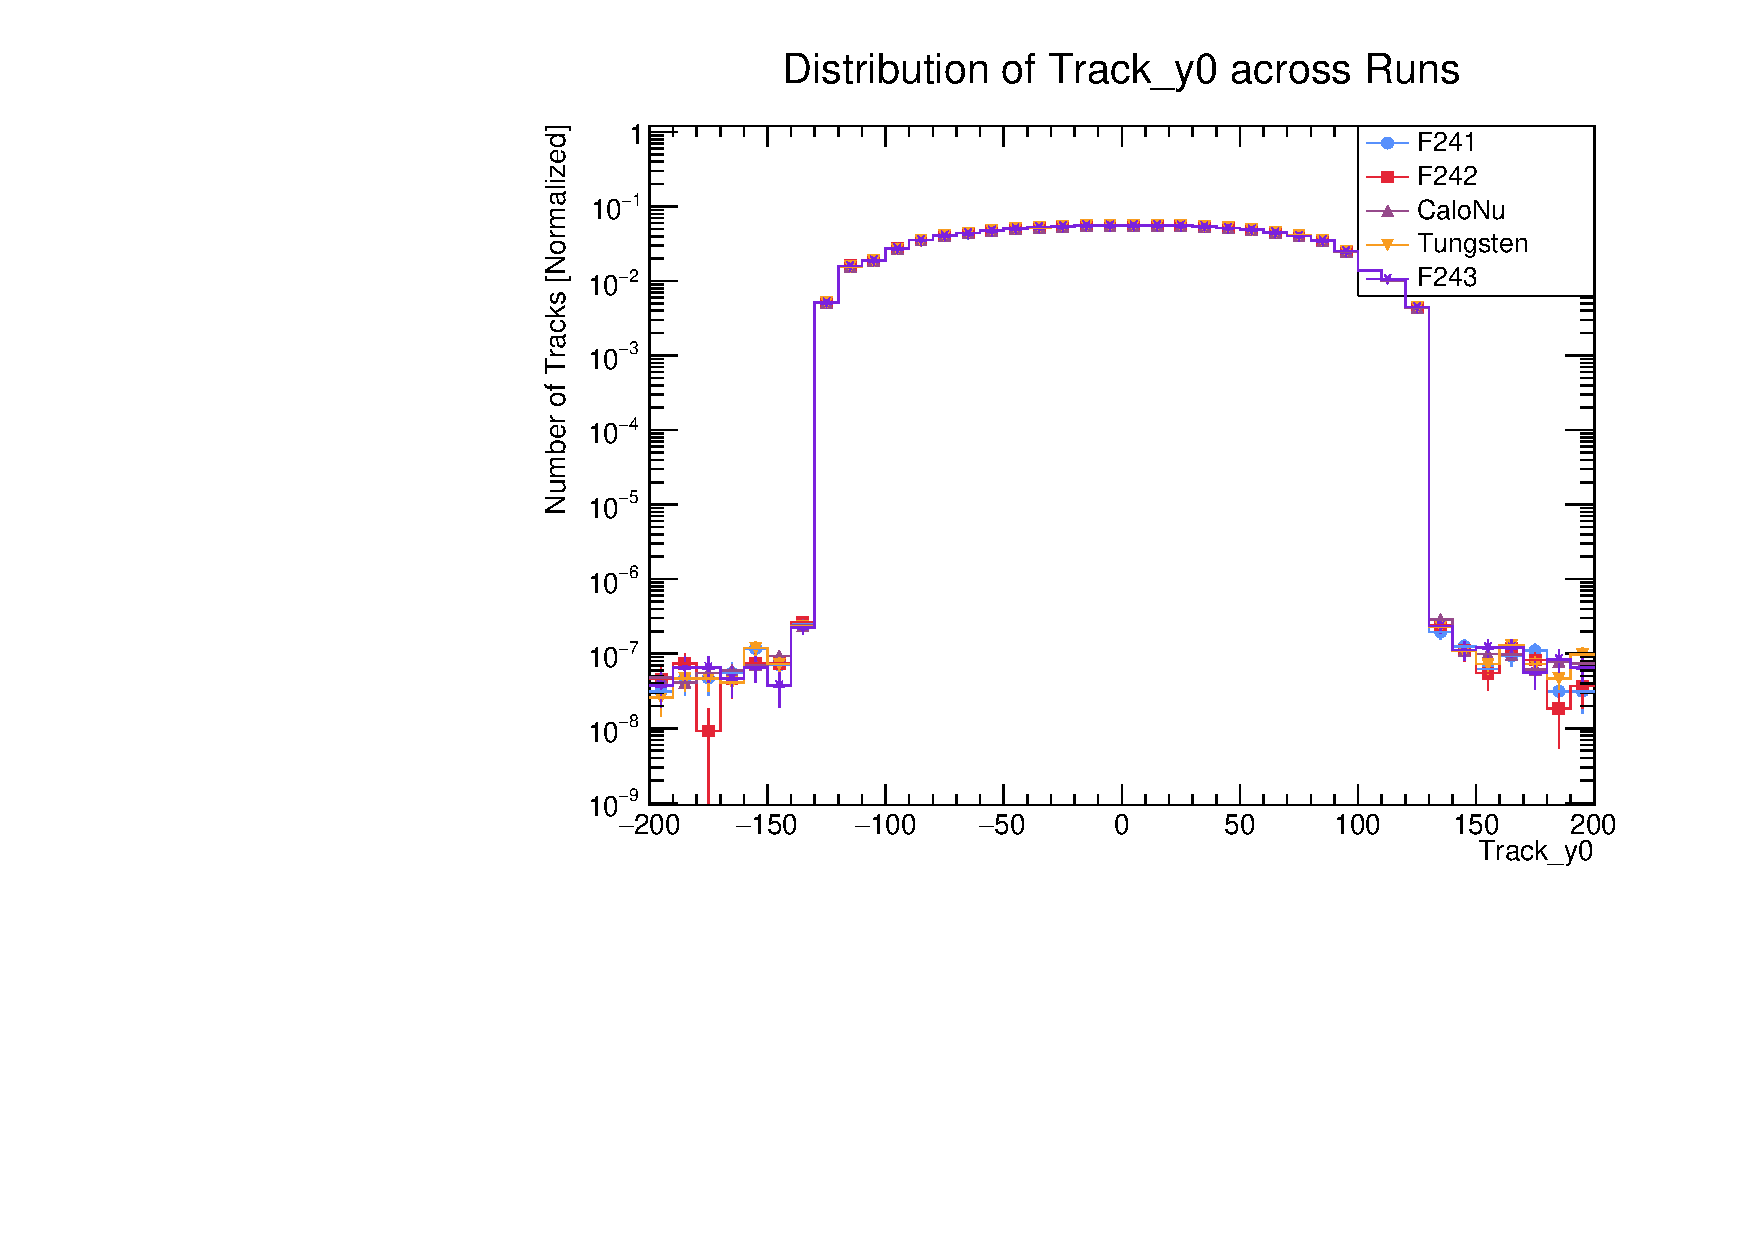
\includegraphics[width=\linewidth]{./RunwisePlots/Track_y0_runwise.pdf}
	\end{figure}
\end{frame}

\begin{frame}{Distribution of Track ThetaX0 across 2024 runs}
	\begin{figure}
		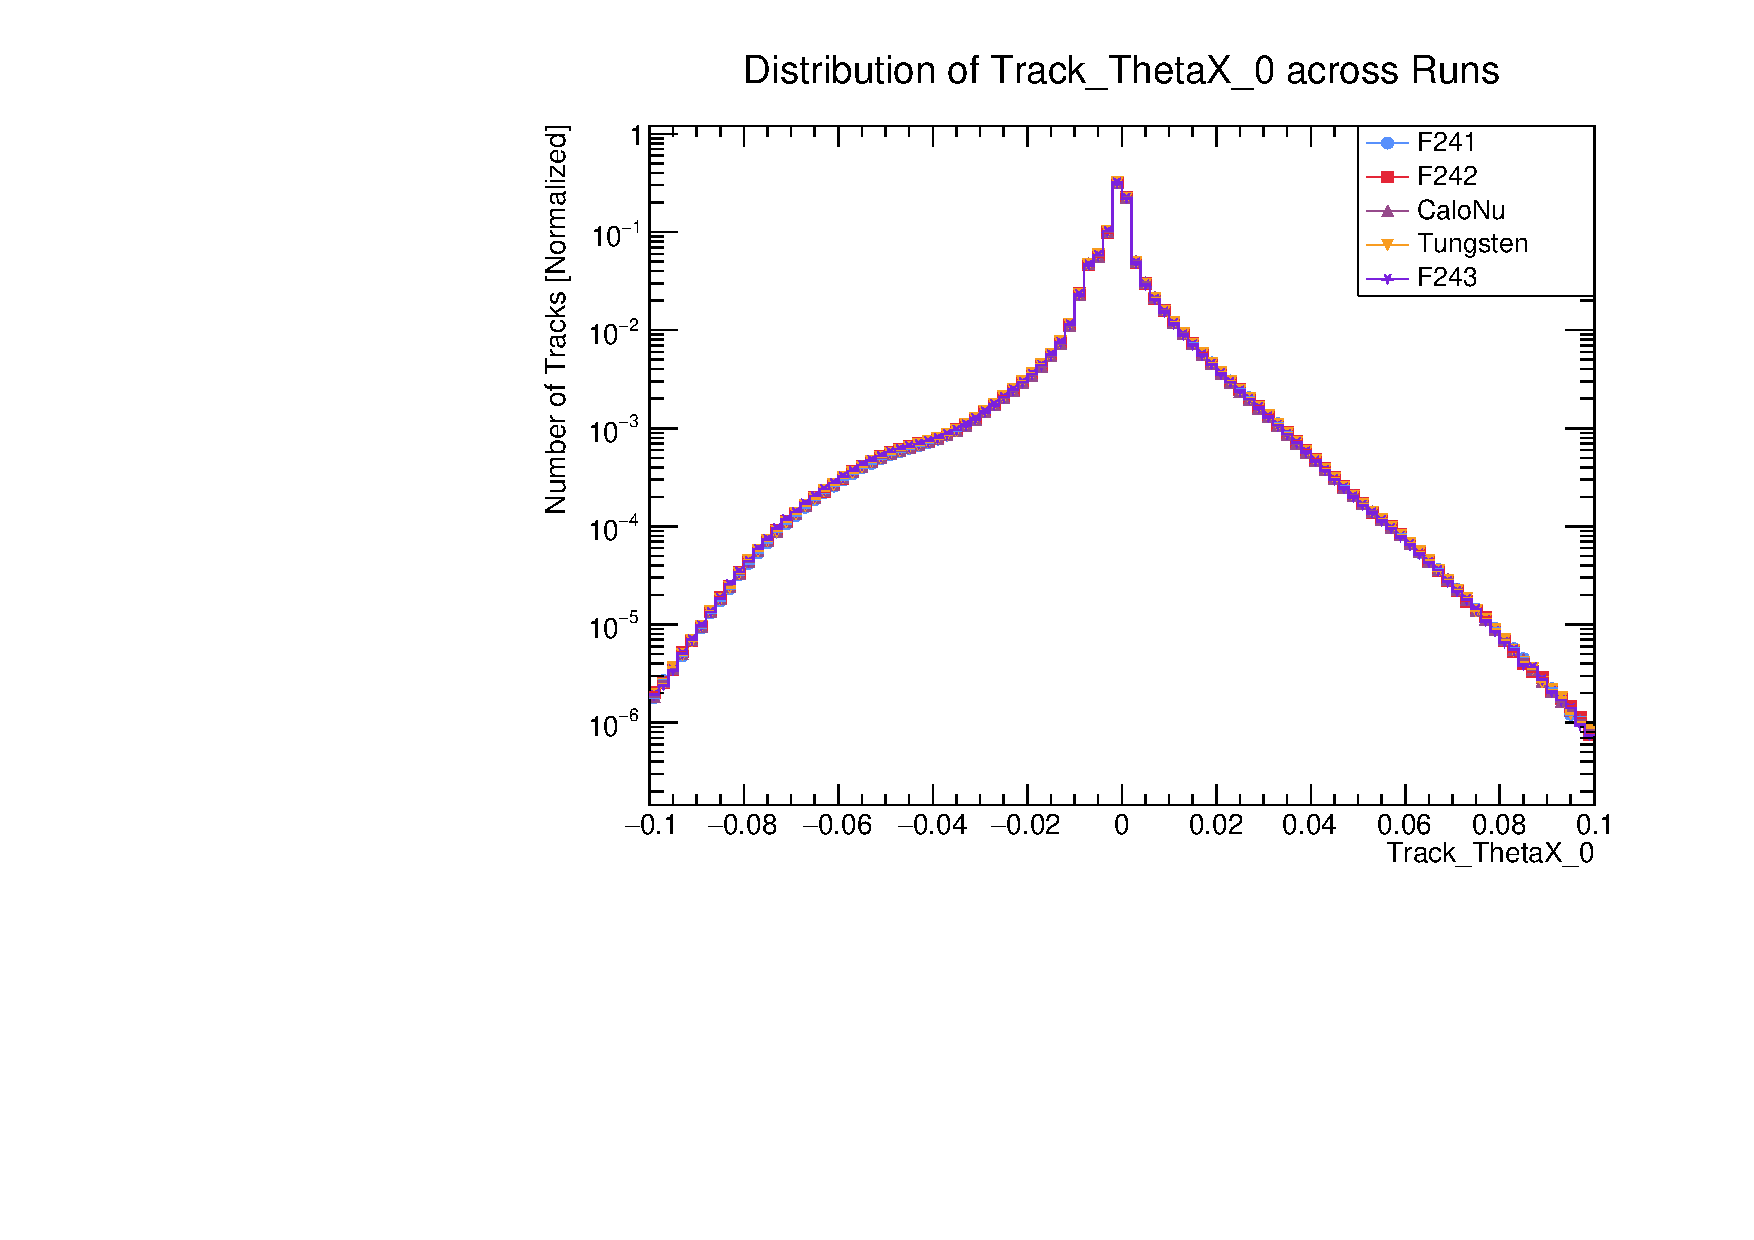
\includegraphics[width=\linewidth]{./RunwisePlots/Track_ThetaX_0_runwise.pdf}
	\end{figure}
\end{frame}
\begin{frame}{Distribution of Track ThetaY0 across runs}
	\begin{figure}
		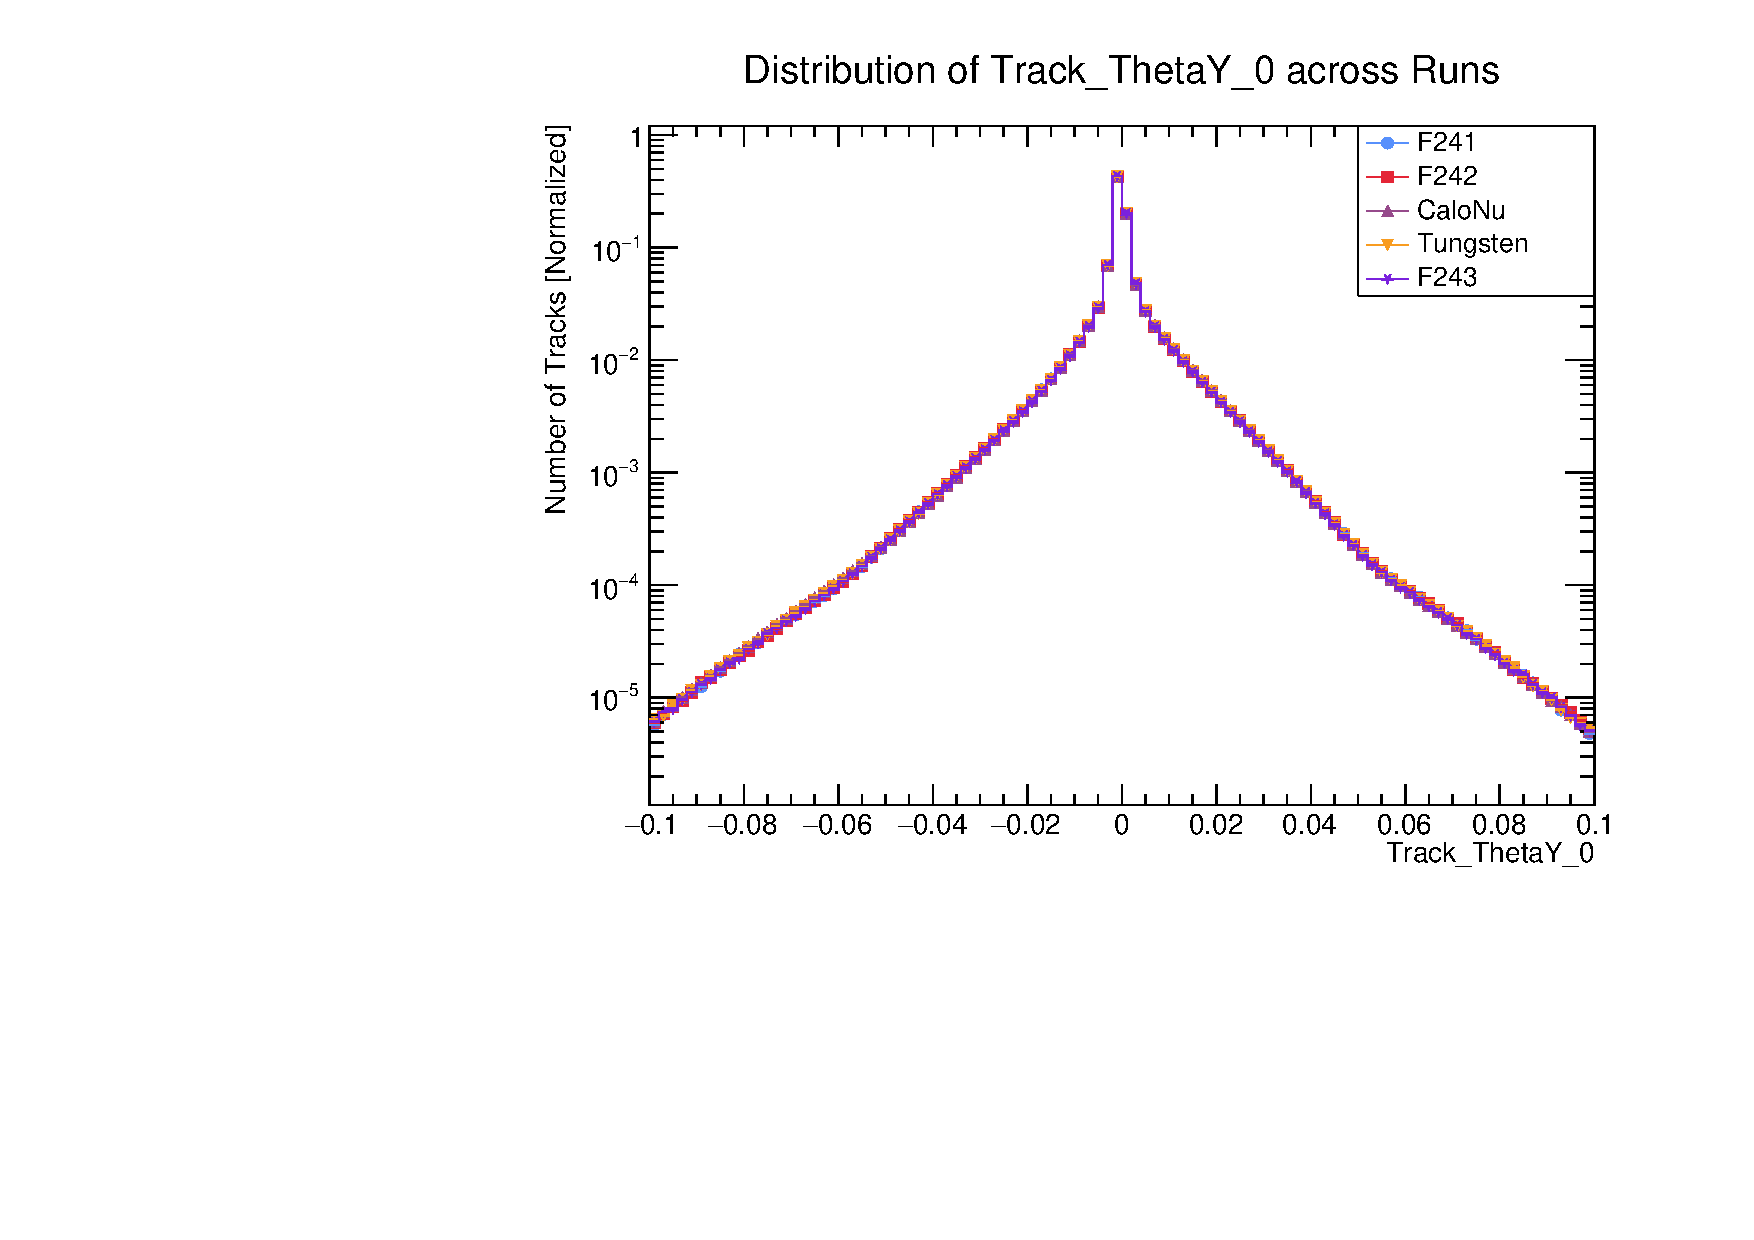
\includegraphics[width=\linewidth]{./RunwisePlots/Track_ThetaY_0_runwise.pdf}
	\end{figure}
\end{frame}

\begin{frame}{Distribution of Track Momenta across runs}
	\begin{figure}
		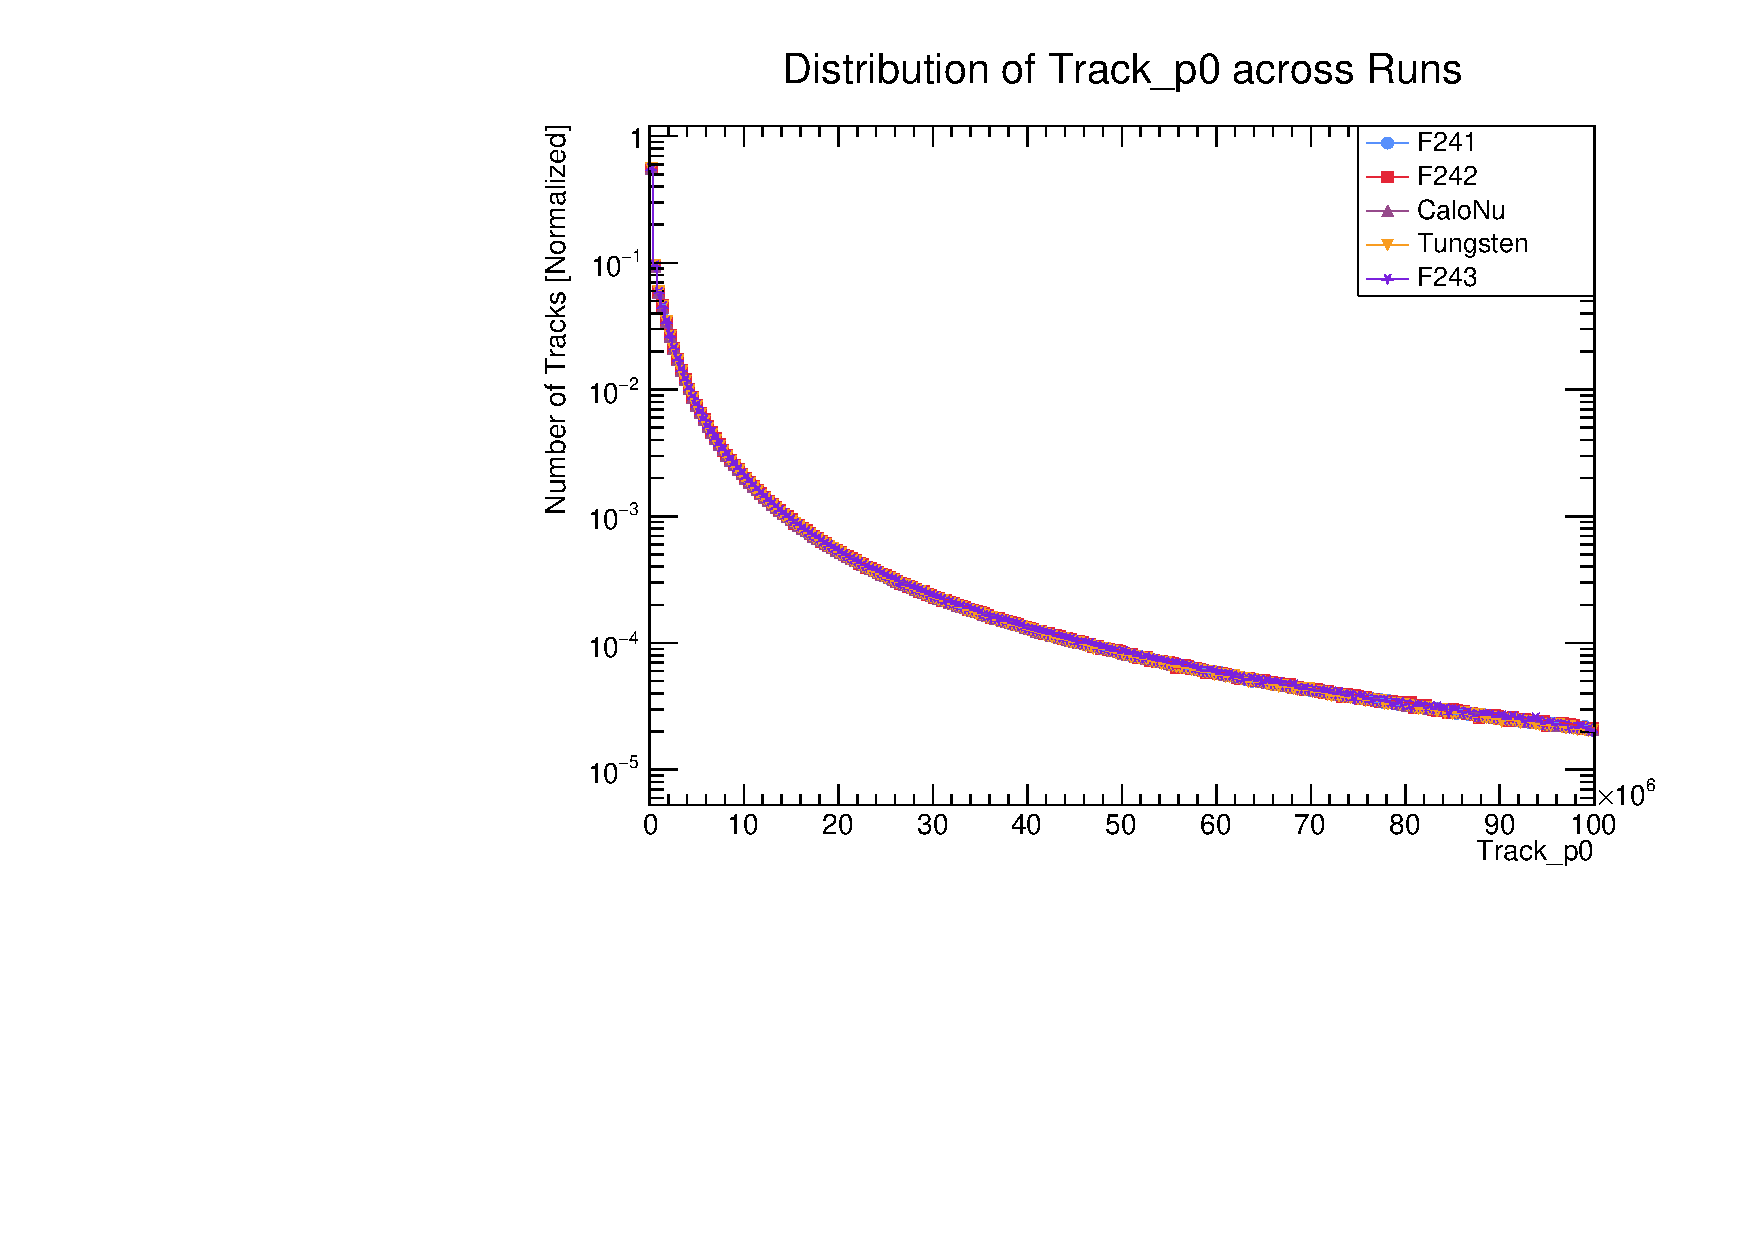
\includegraphics[width=\linewidth]{./RunwisePlots/Track_p0_runwise.pdf}
	\end{figure}
\end{frame}

\begin{frame}{longTracks across 2024 runs}
	\begin{columns}
		\begin{column}{0.55 \linewidth}
			\begin{figure}
				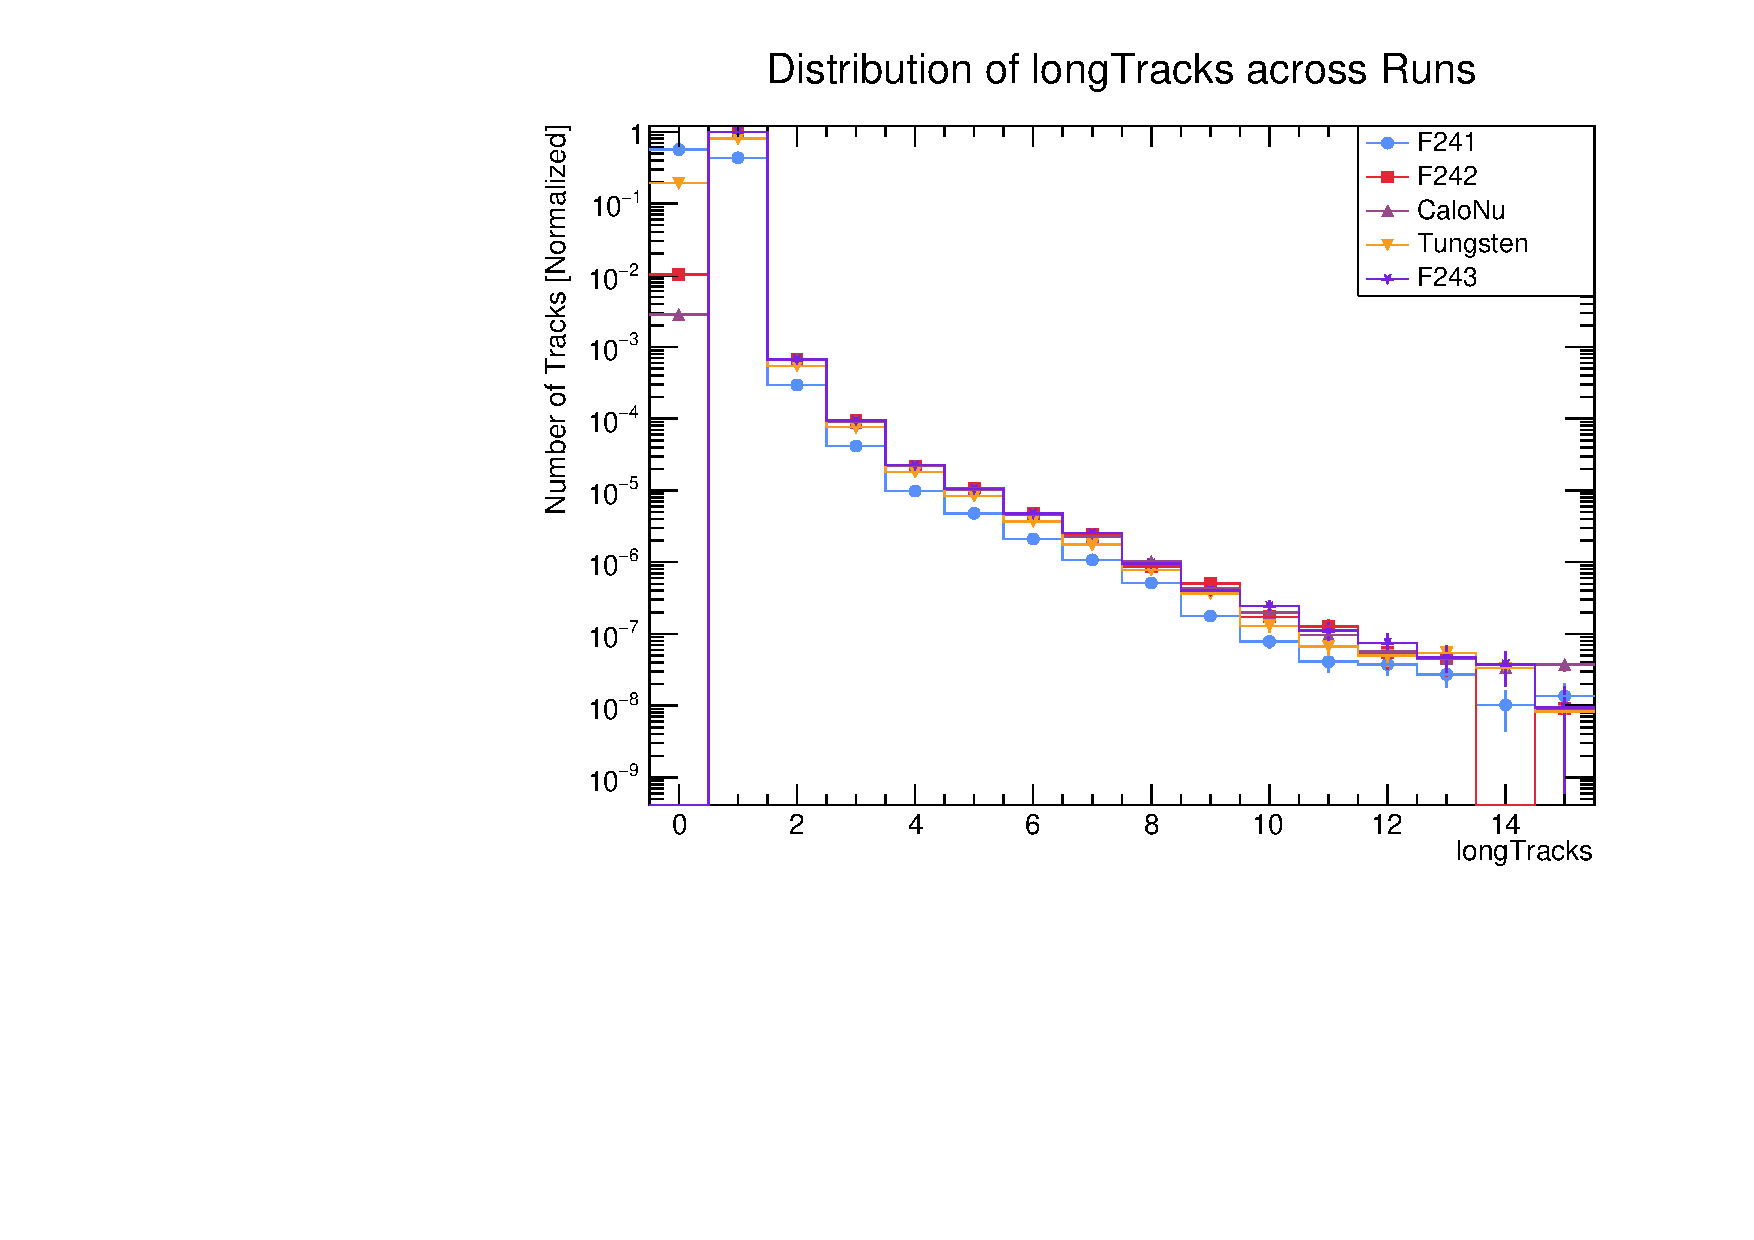
\includegraphics[width=\linewidth]{./RunwisePlots/longTracks_runwise.pdf}
				\caption{LongTracks across 2024 runs [Normalized to Sum of Entries across all bins]}
			\end{figure}
		\end{column}
		\begin{column}{0.55 \linewidth}
			\begin{figure}
				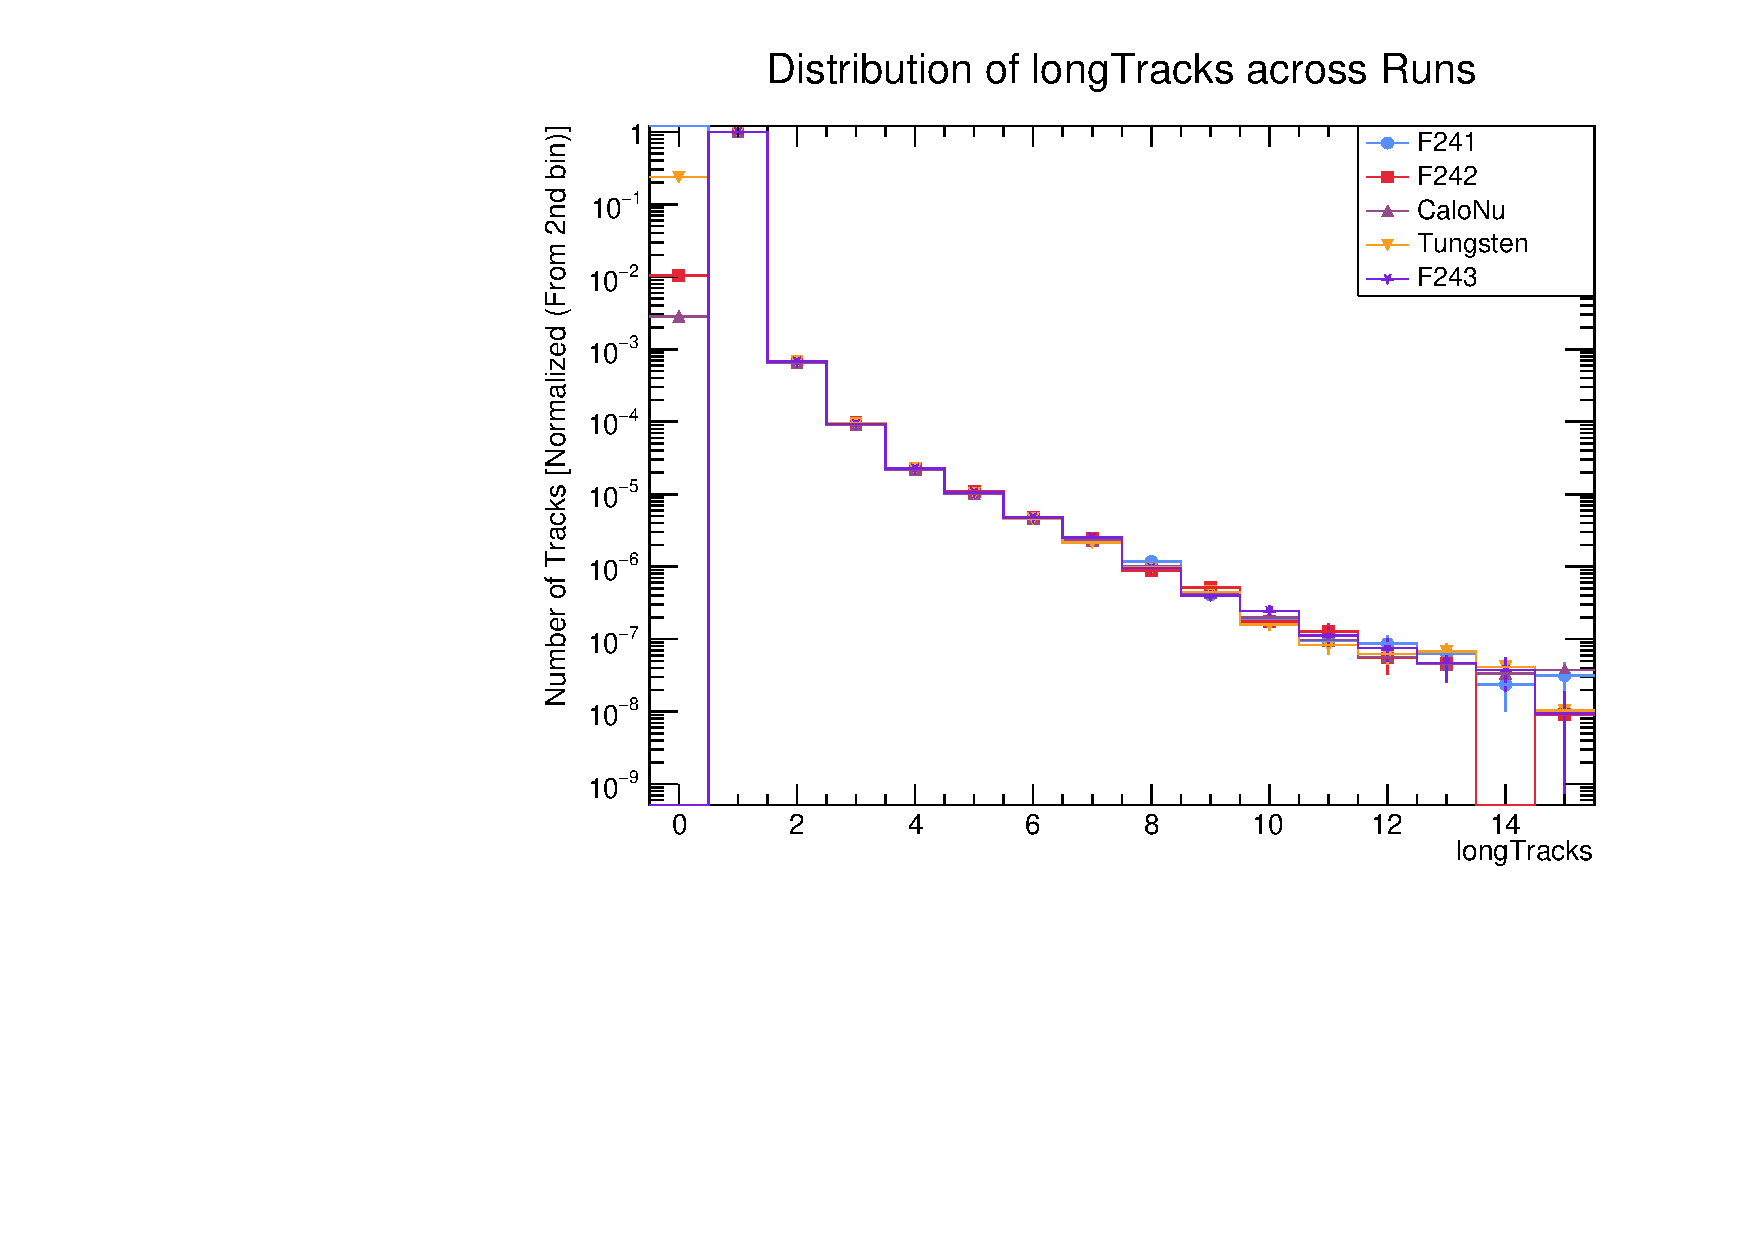
\includegraphics[width=\linewidth]{RunwisePlots/longTracks_normalisedfrom2_runwise.pdf}
				\caption{LongTracks across 2024 runs [Normalized to Sum of Entries starting from 2nd bin]}
			\end{figure}
		\end{column}
	\end{columns}
	\begin{itemize}
		\item F241 seems to show a higher number of 0-longTrack events.
	\end{itemize}
	% \begin{figure}
	% 	\begin{subfigure}{0.45\linewidth}
	% 		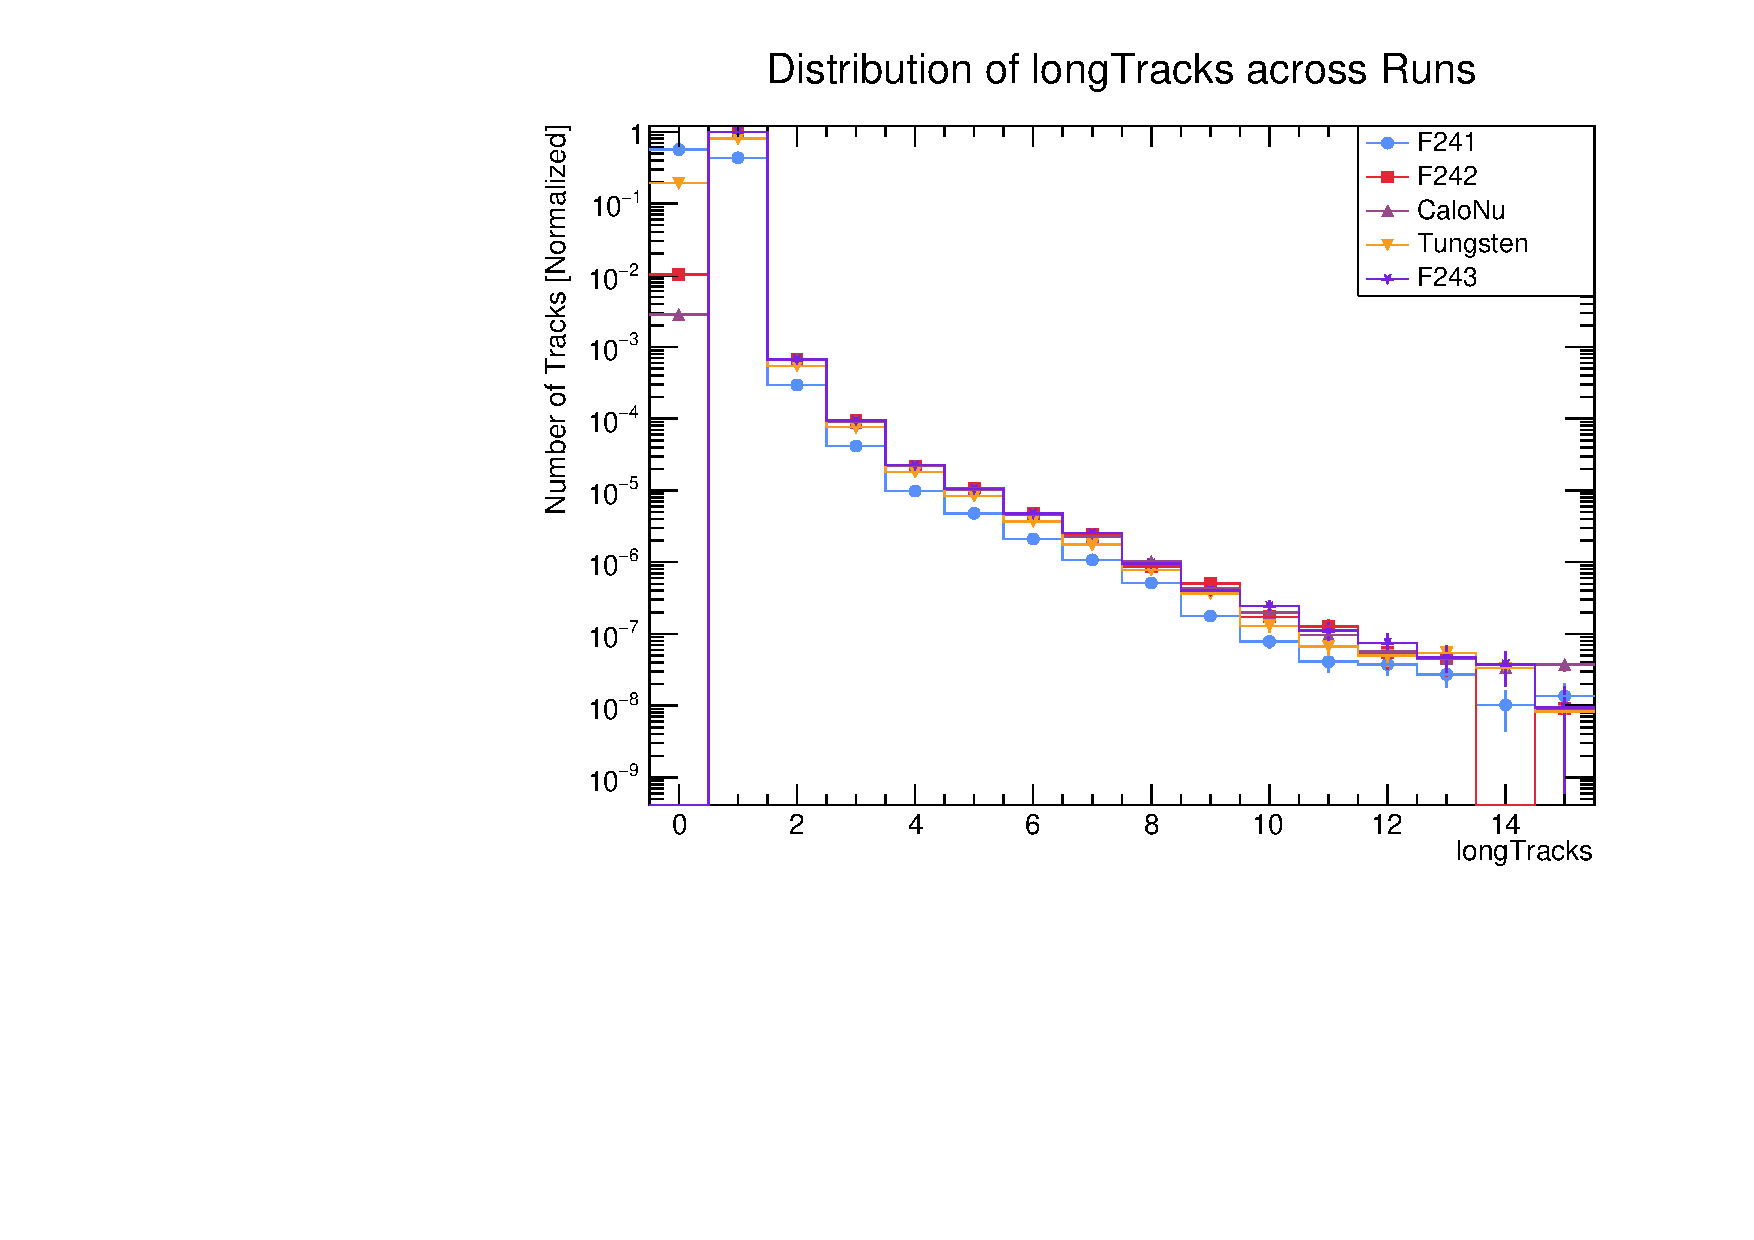
\includegraphics[width=1.2\linewidth]{./RunwisePlots/longTracks_runwise.pdf}
	% 	\end{subfigure}
	% 	\begin{subfigure}{0.45\linewidth}
	% 		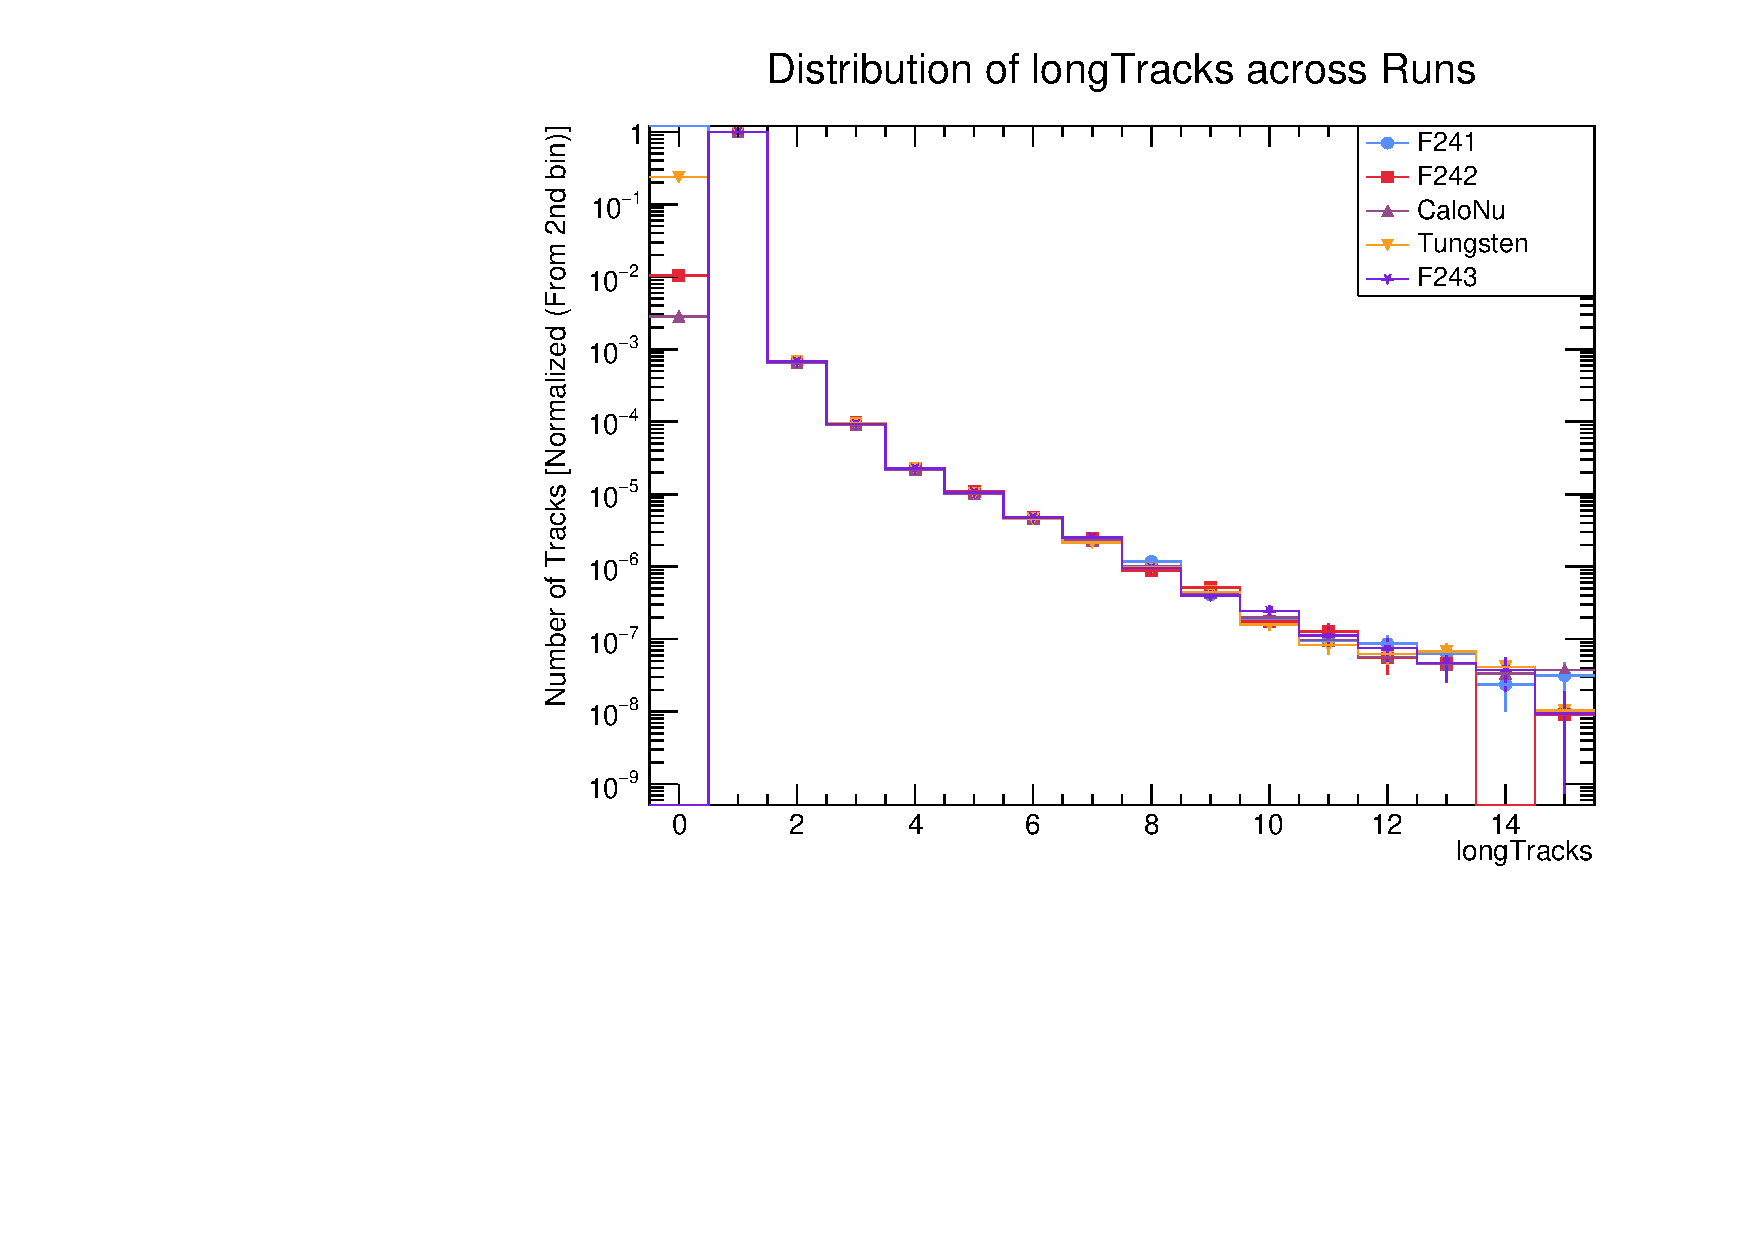
\includegraphics[width=1.2\linewidth]{RunwisePlots/longTracks_normalisedfrom2_runwise.pdf}
	% 	\end{subfigure}
	% \end{figure}
\end{frame}

\begin{frame}{Track Charge across 2024 runs}
	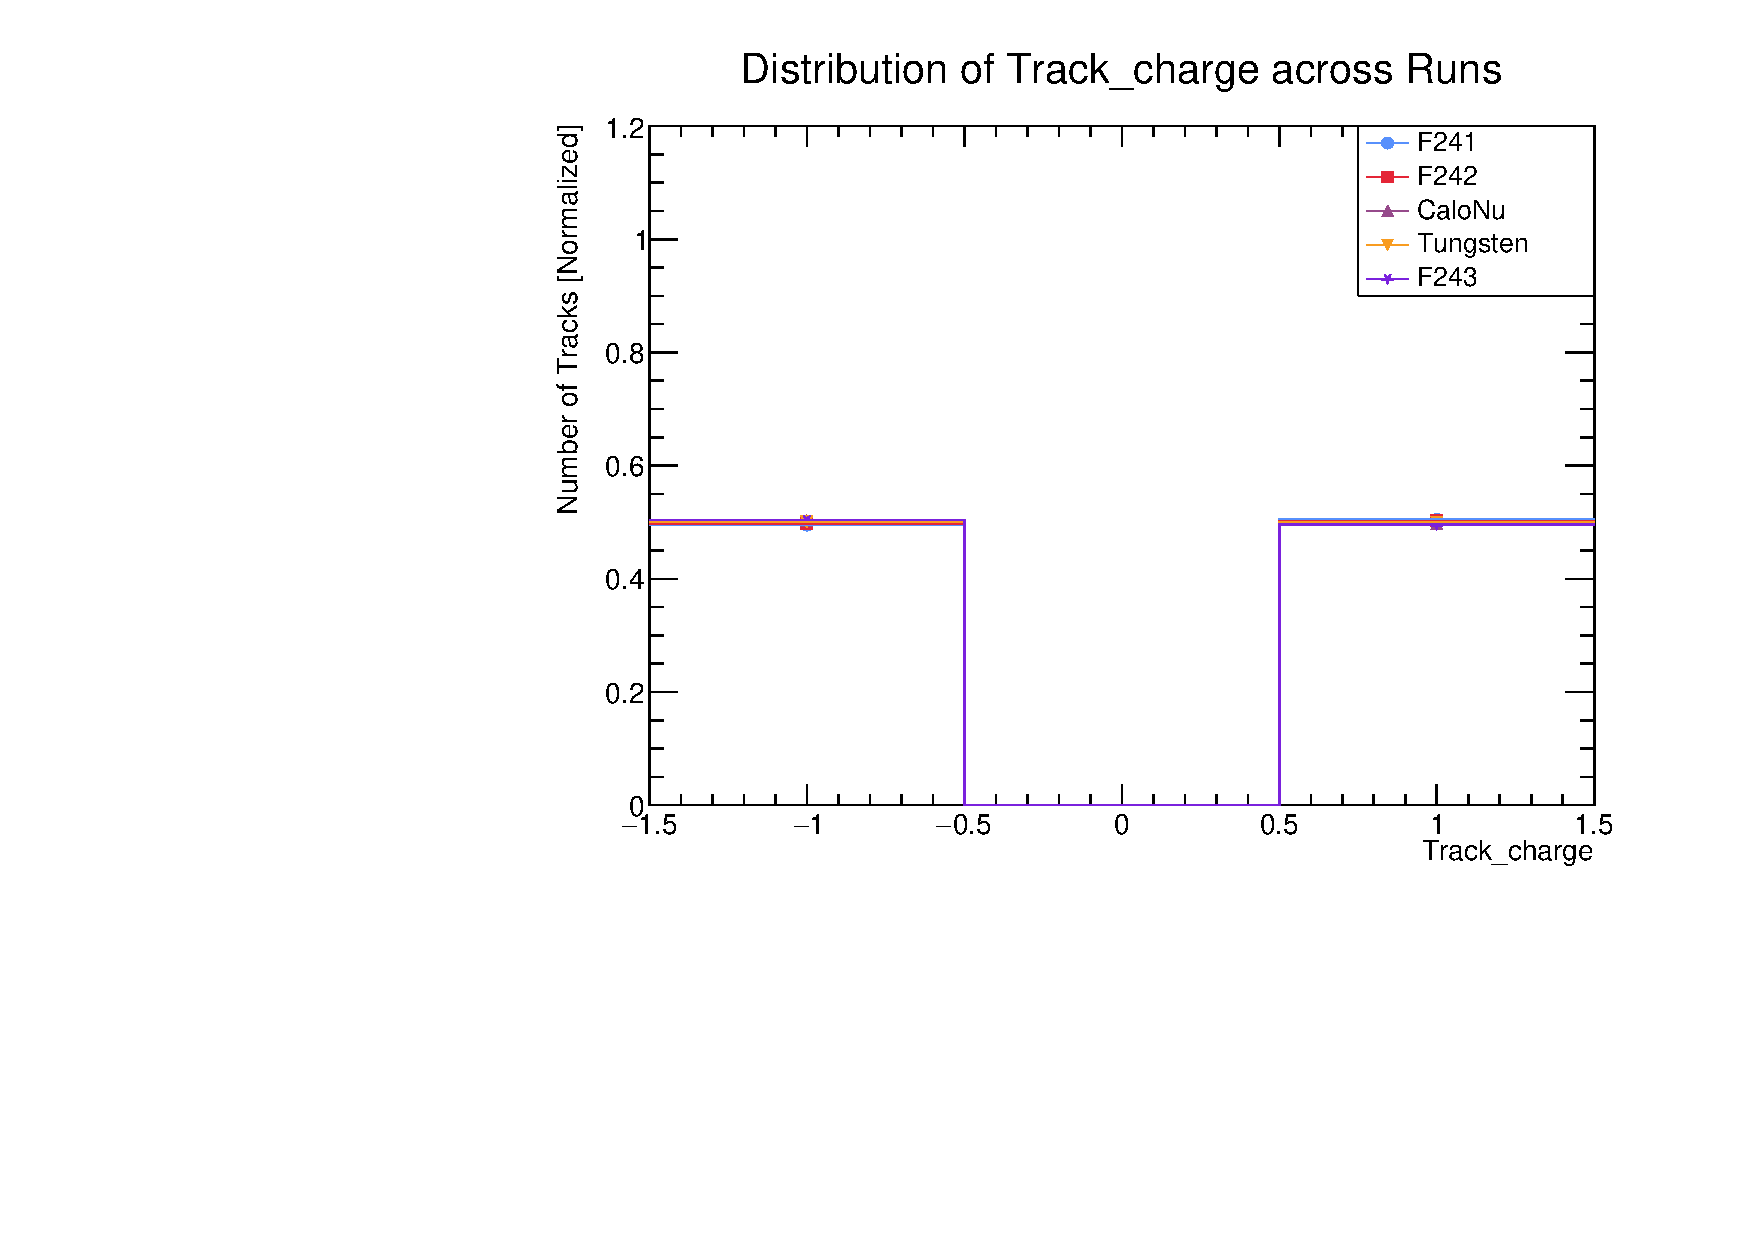
\includegraphics[width=\linewidth]{./RunwisePlots/Track_charge_runwise.pdf}
\end{frame}

\begin{frame}{Track Chi2 across 2024 runs}
	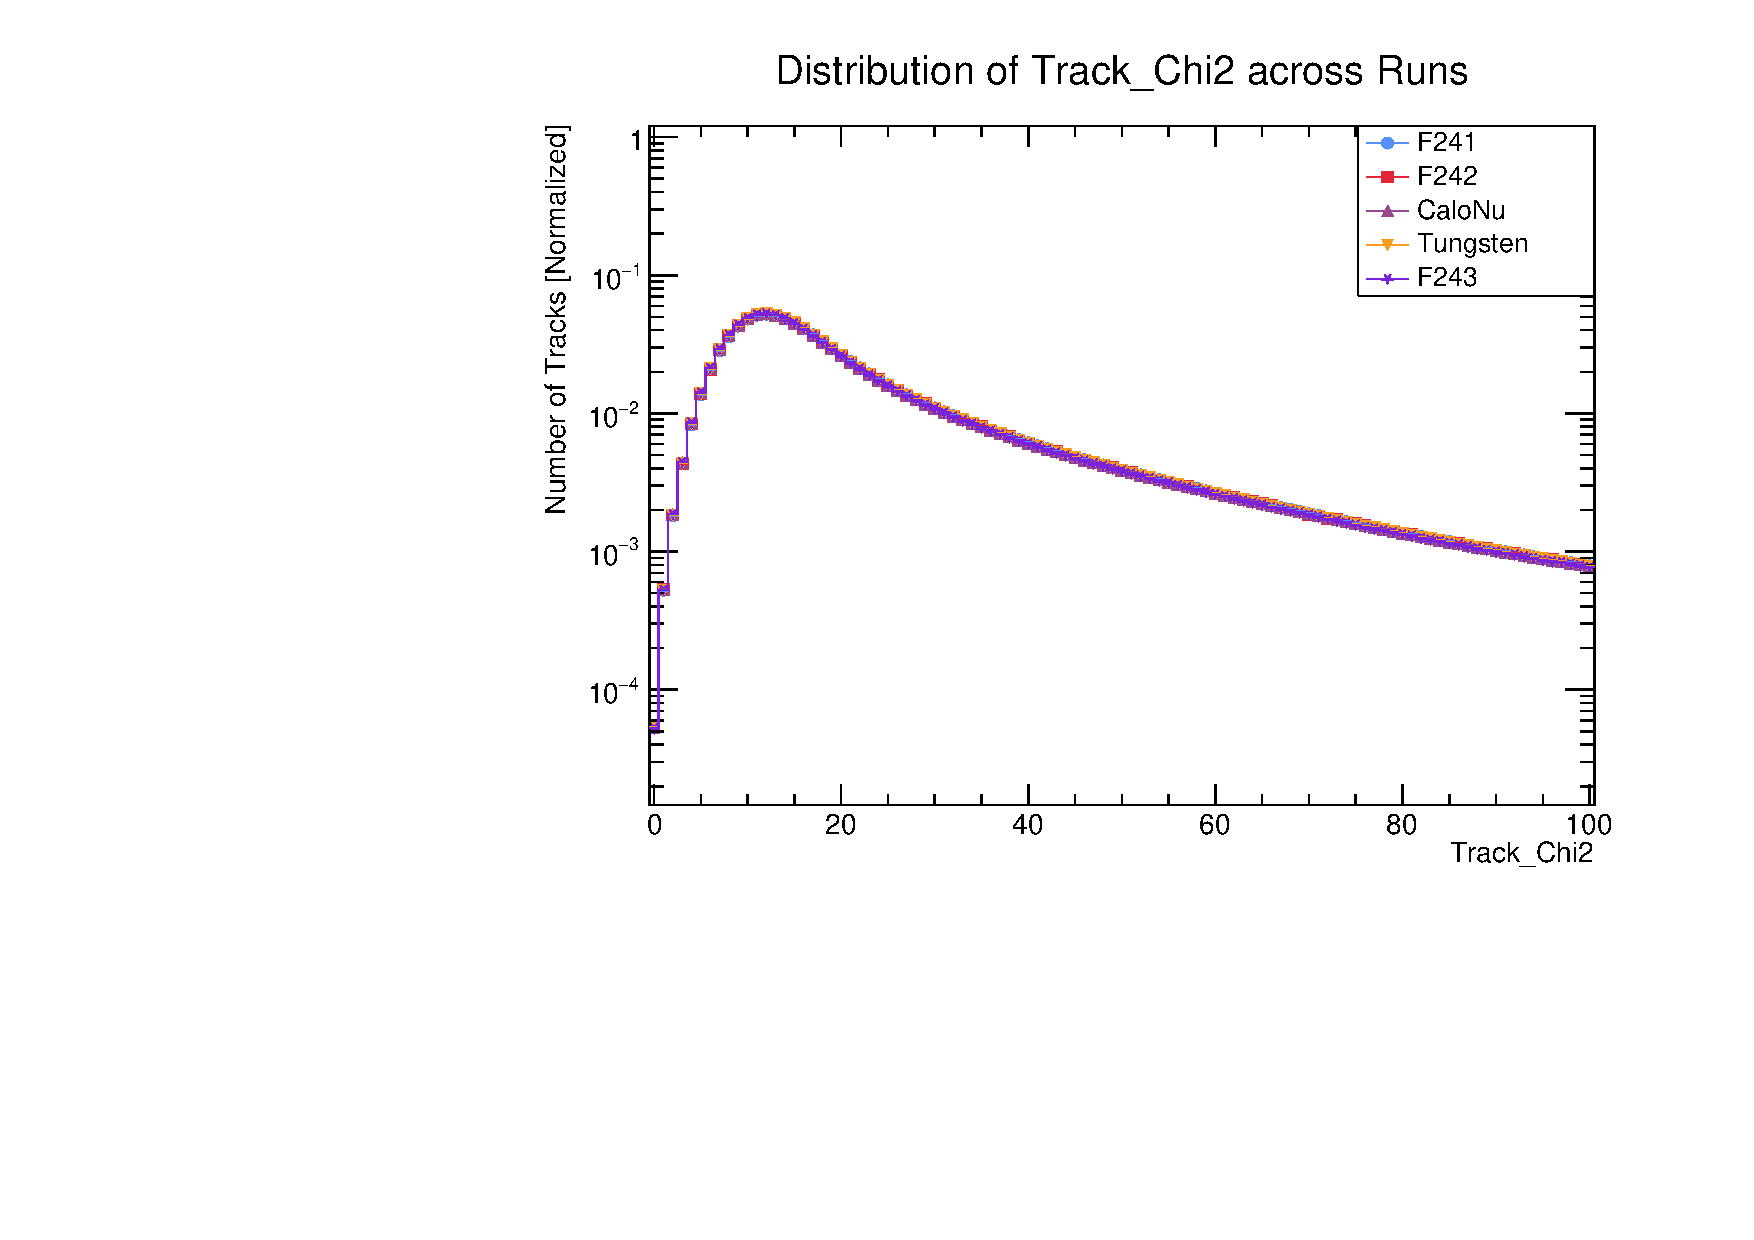
\includegraphics[width=\linewidth]{./RunwisePlots/Track_Chi2_runwise.pdf}
\end{frame}

\begin{frame}{Track nDoF across 2024 runs}
	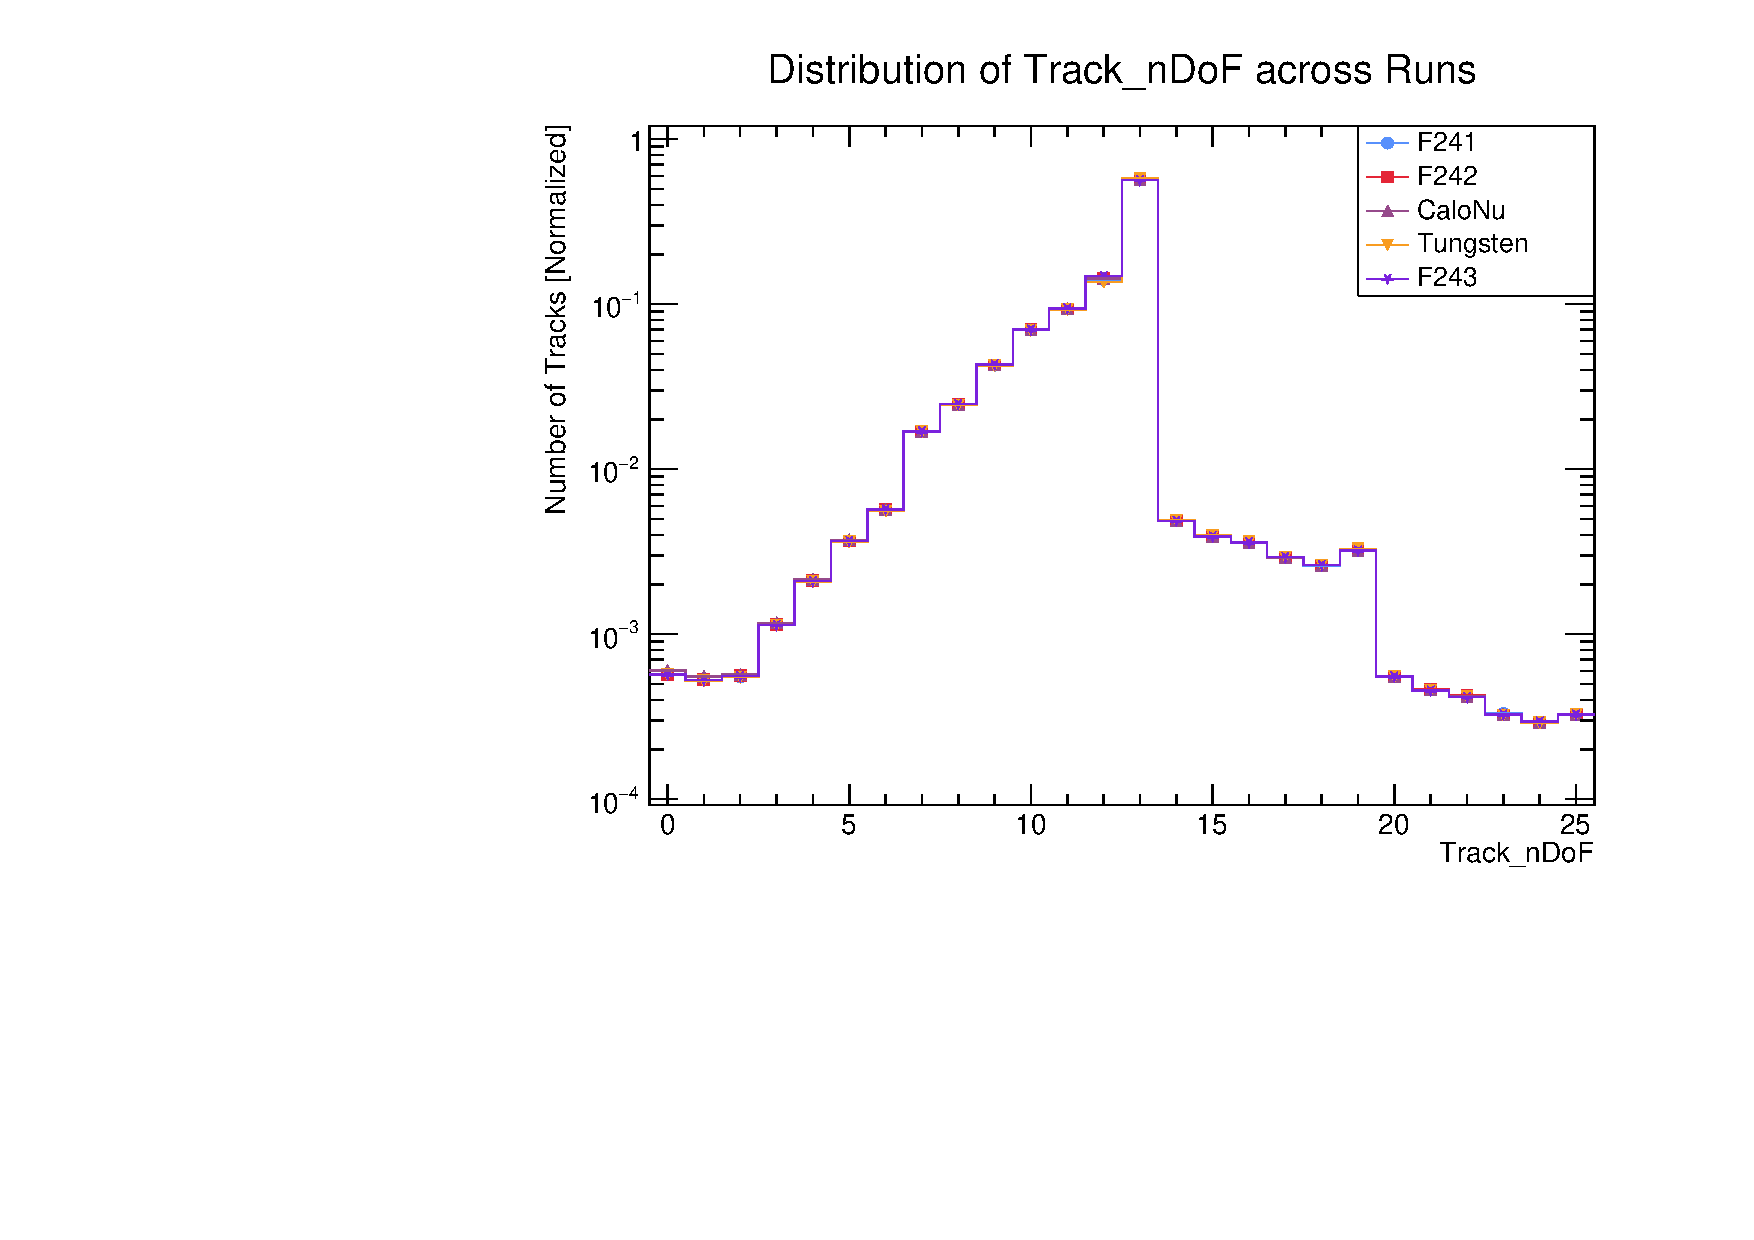
\includegraphics[width=\linewidth]{./RunwisePlots/Track_nDoF_runwise.pdf}
\end{frame}

\begin{frame}{Track Chi2perDoF across 2024 runs}
	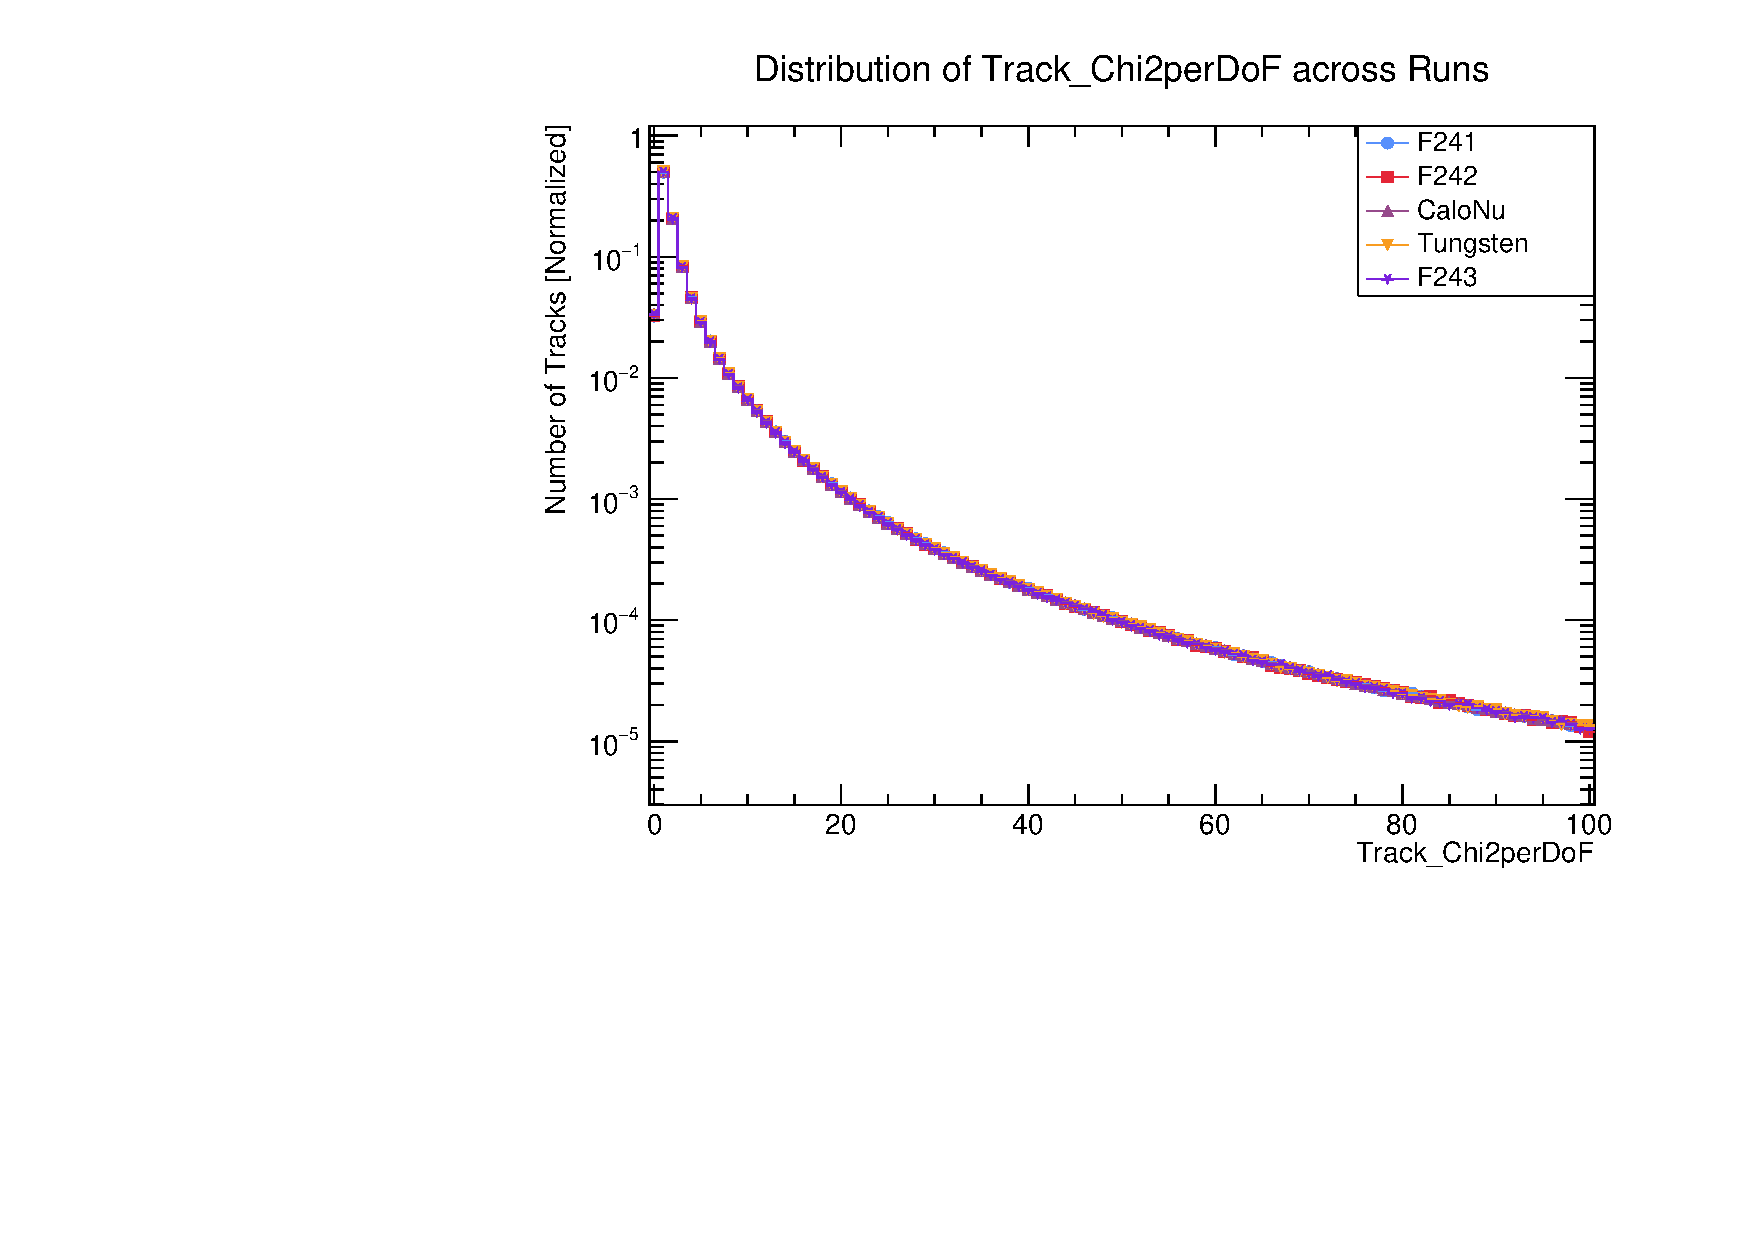
\includegraphics[width=\linewidth]{./RunwisePlots/Track_Chi2perDoF_runwise.pdf}
\end{frame}

\begin{frame}{Track nLayers across 2024 runs}
	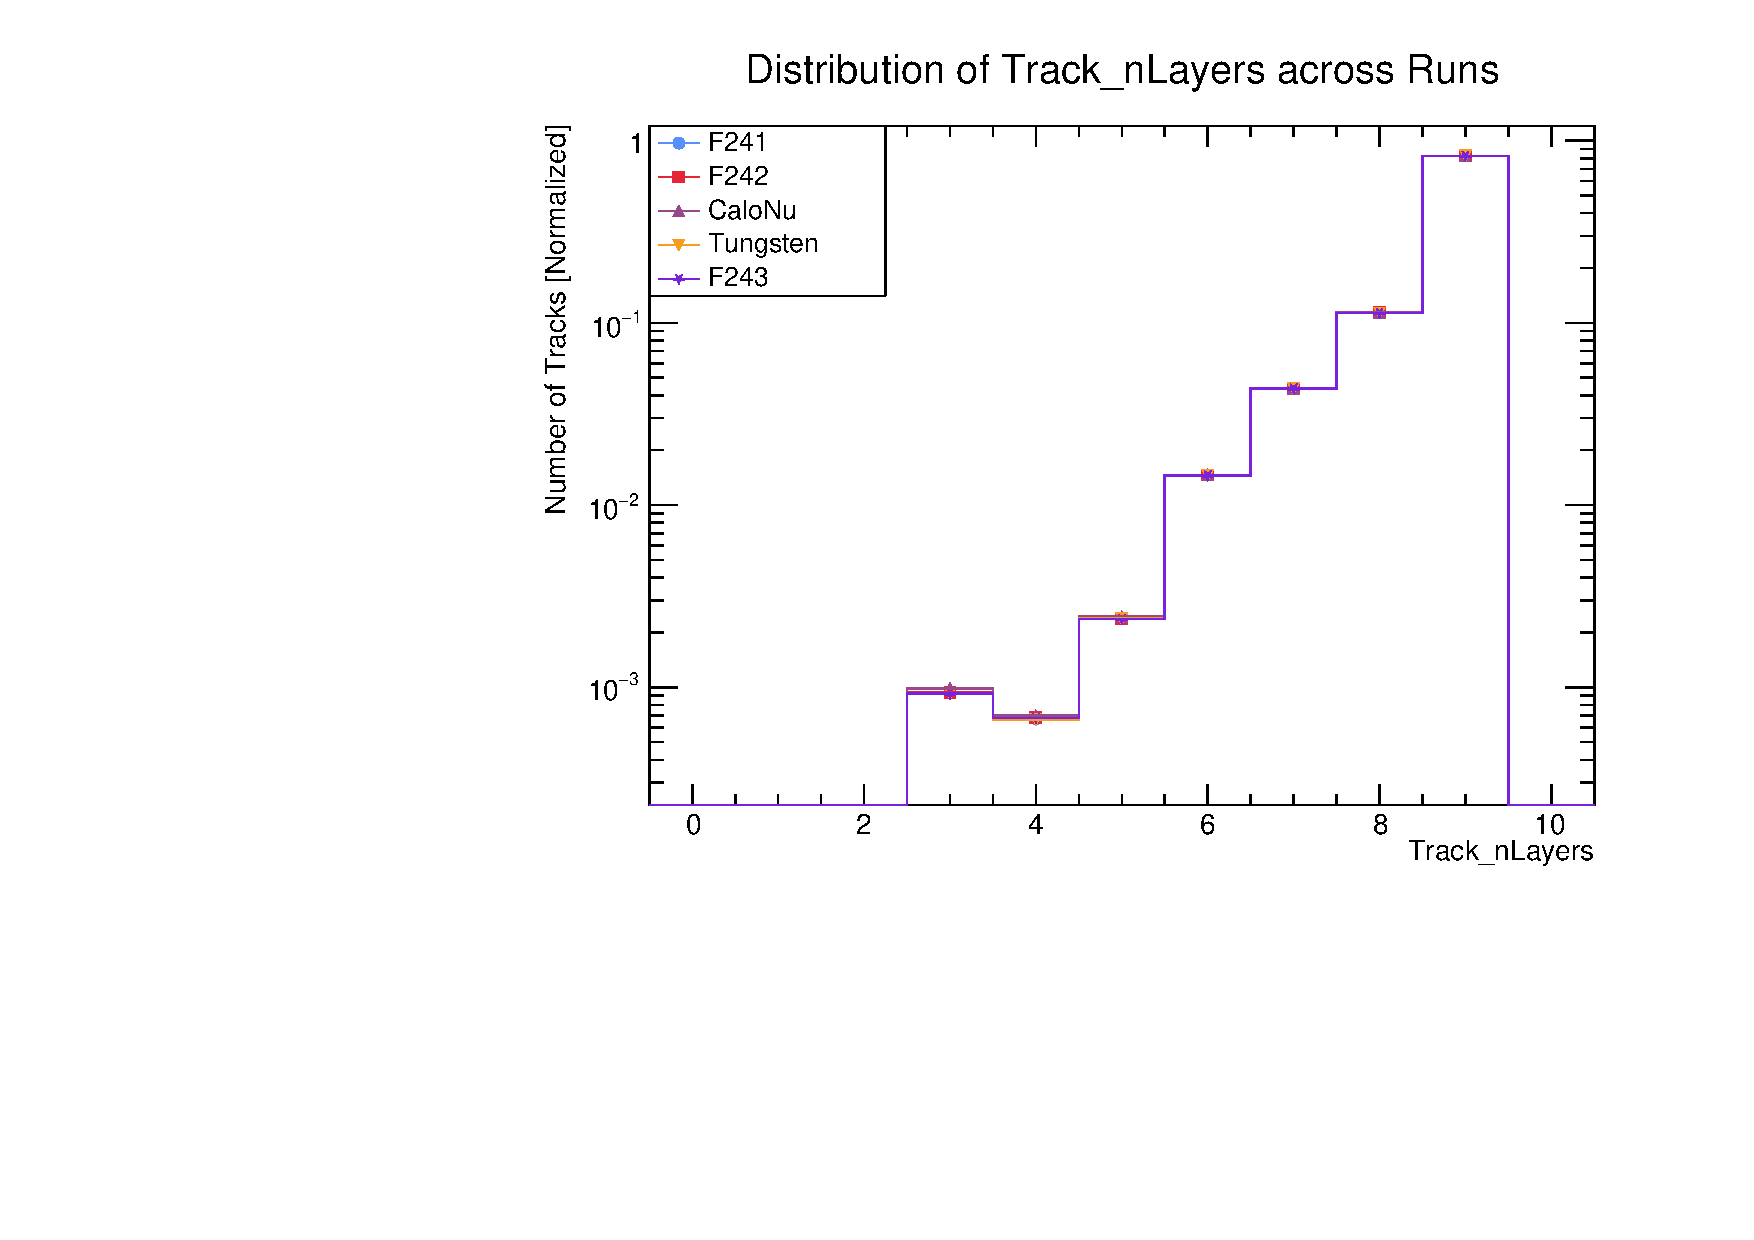
\includegraphics[width=\linewidth]{./RunwisePlots/Track_nLayers_runwise.pdf}
\end{frame}

